\documentclass[]{revtex4}\usepackage[]{graphicx}\usepackage[]{color}
%% maxwidth is the original width if it is less than linewidth
%% otherwise use linewidth (to make sure the graphics do not exceed the margin)
\makeatletter
\def\maxwidth{ %
  \ifdim\Gin@nat@width>\linewidth
    \linewidth
  \else
    \Gin@nat@width
  \fi
}
\makeatother

\definecolor{fgcolor}{rgb}{0.345, 0.345, 0.345}
\newcommand{\hlnum}[1]{\textcolor[rgb]{0.686,0.059,0.569}{#1}}%
\newcommand{\hlstr}[1]{\textcolor[rgb]{0.192,0.494,0.8}{#1}}%
\newcommand{\hlcom}[1]{\textcolor[rgb]{0.678,0.584,0.686}{\textit{#1}}}%
\newcommand{\hlopt}[1]{\textcolor[rgb]{0,0,0}{#1}}%
\newcommand{\hlstd}[1]{\textcolor[rgb]{0.345,0.345,0.345}{#1}}%
\newcommand{\hlkwa}[1]{\textcolor[rgb]{0.161,0.373,0.58}{\textbf{#1}}}%
\newcommand{\hlkwb}[1]{\textcolor[rgb]{0.69,0.353,0.396}{#1}}%
\newcommand{\hlkwc}[1]{\textcolor[rgb]{0.333,0.667,0.333}{#1}}%
\newcommand{\hlkwd}[1]{\textcolor[rgb]{0.737,0.353,0.396}{\textbf{#1}}}%

\usepackage{framed}
\makeatletter
\newenvironment{kframe}{%
 \def\at@end@of@kframe{}%
 \ifinner\ifhmode%
  \def\at@end@of@kframe{\end{minipage}}%
  \begin{minipage}{\columnwidth}%
 \fi\fi%
 \def\FrameCommand##1{\hskip\@totalleftmargin \hskip-\fboxsep
 \colorbox{shadecolor}{##1}\hskip-\fboxsep
     % There is no \\@totalrightmargin, so:
     \hskip-\linewidth \hskip-\@totalleftmargin \hskip\columnwidth}%
 \MakeFramed {\advance\hsize-\width
   \@totalleftmargin\z@ \linewidth\hsize
   \@setminipage}}%
 {\par\unskip\endMakeFramed%
 \at@end@of@kframe}
\makeatother

\definecolor{shadecolor}{rgb}{.97, .97, .97}
\definecolor{messagecolor}{rgb}{0, 0, 0}
\definecolor{warningcolor}{rgb}{1, 0, 1}
\definecolor{errorcolor}{rgb}{1, 0, 0}
\newenvironment{knitrout}{}{} % an empty environment to be redefined in TeX

\usepackage{alltt} %twocolumn revtex4
\usepackage[T1]{fontenc}
\usepackage{lmodern}
\usepackage{booktabs}
\IfFileExists{upquote.sty}{\usepackage{upquote}}{}
\begin{document}

\title{Simulated tree clustered by UCSD soft. - Feb 2016}
\author{S. Le Vu}
%\affiliation{ICL}
\date{\today}

\maketitle





\section{Intro}
\begin{itemize}
\item "time-based" distances have been extracted form simulated coalescent tree
\item distances normalized from 0 to 1
\end{itemize}
%' 
%' << get distances, results='asis', echo = FALSE>>=
%' @
\begin{center}
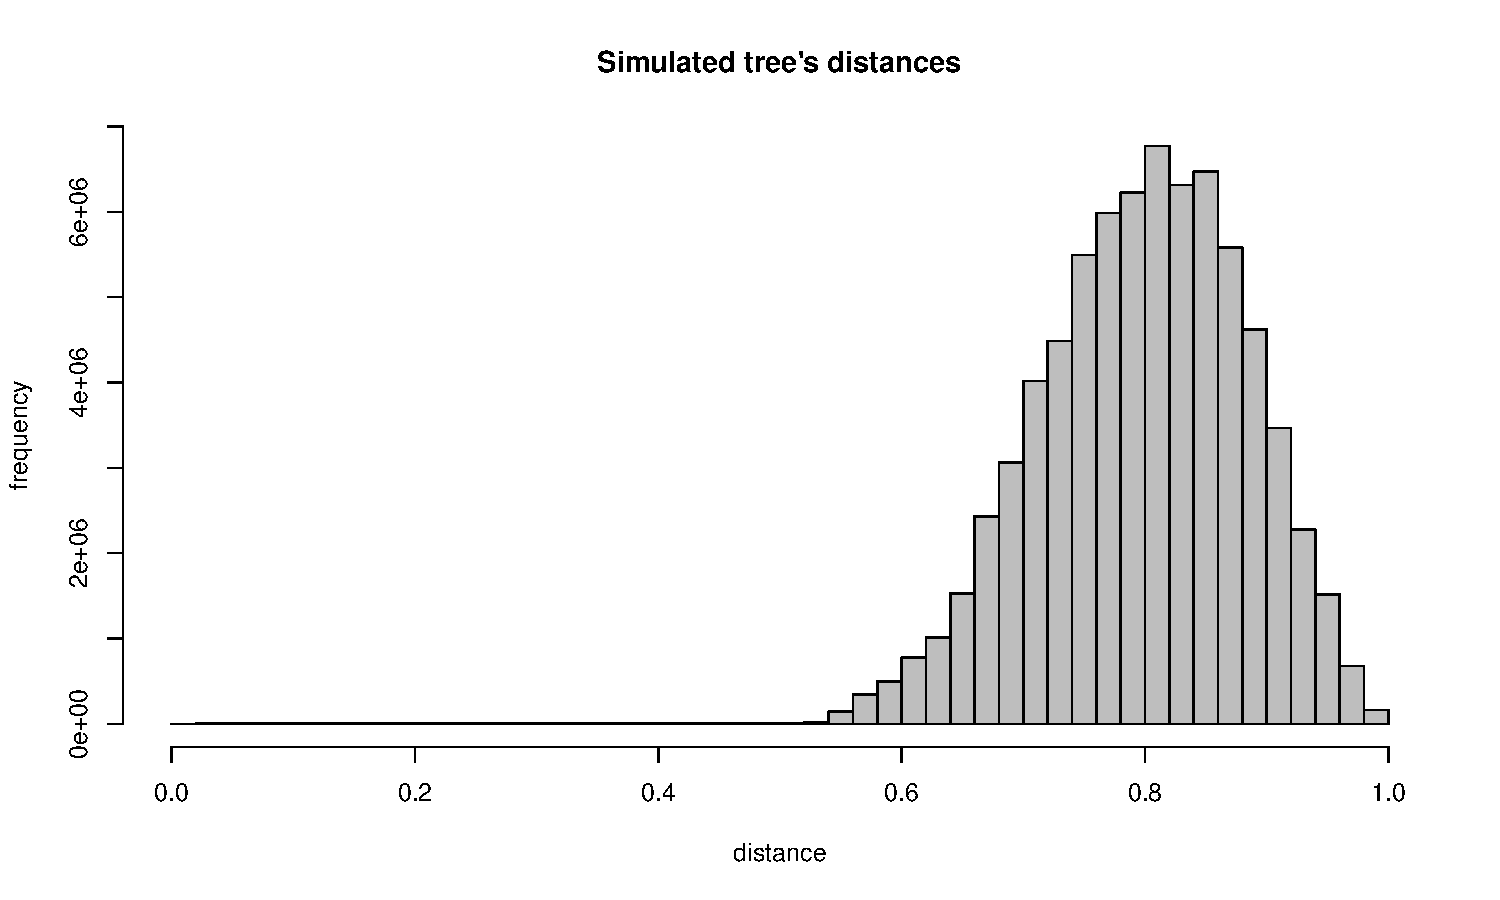
\includegraphics[scale=0.4]{figure/plotget_distances-1.pdf}
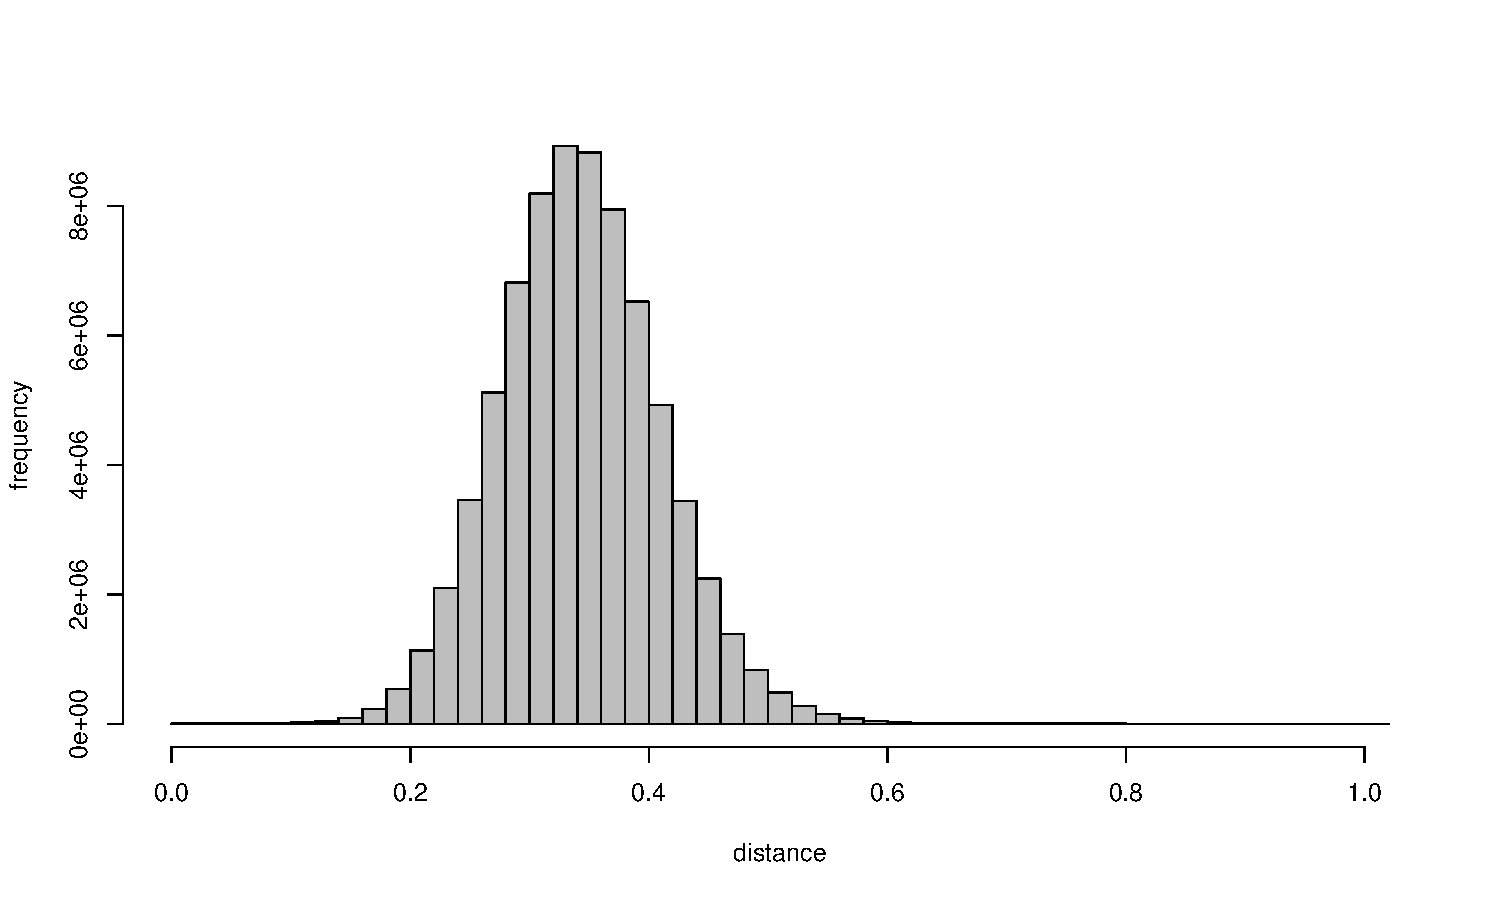
\includegraphics[scale=0.4]{figure/plotget_distances-2.pdf}
\end{center}



\section{UCSD hivclustering}
Read saved results from UCSD \textsf{hivclustering}
\begin{knitrout}
\definecolor{shadecolor}{rgb}{0.969, 0.969, 0.969}\color{fgcolor}\begin{kframe}
\begin{alltt}
\hlcom{### only cluster members}
\hlstd{simclus} \hlkwb{<-} \hlkwd{readRDS}\hlstd{(}\hlkwc{file} \hlstd{=} \hlstr{"data/simclus.rds"}\hlstd{)[[}\hlnum{3}\hlstd{]]}
\hlstd{ukclus} \hlkwb{<-} \hlkwd{readRDS}\hlstd{(}\hlkwc{file} \hlstd{=} \hlstr{"data/ukclus.rds"}\hlstd{)[[}\hlnum{3}\hlstd{]]}
\end{alltt}
\end{kframe}
\end{knitrout}


To construct clusters, threshold were determined by quantiles of distances (0.05\%, 0.1\%, 1\% and 10\%). For simulated and UK trees
\begin{knitrout}
\definecolor{shadecolor}{rgb}{0.969, 0.969, 0.969}\color{fgcolor}\begin{kframe}
\begin{alltt}
\hlcom{## read saved results of UCSD clustering}
\hlkwd{readRDS}\hlstd{(}\hlkwc{file} \hlstd{=} \hlstr{"data/simclus.rds"}\hlstd{)[[}\hlnum{1}\hlstd{]]}
\end{alltt}
\begin{verbatim}
    0.05%      0.1%        1%       10%       25%       50% 
0.2340219 0.5334507 0.5870679 0.6843790 0.7404369 0.8025368 
\end{verbatim}
\begin{alltt}
\hlkwd{readRDS}\hlstd{(}\hlkwc{file} \hlstd{=} \hlstr{"data/ukclus.rds"}\hlstd{)[[}\hlnum{1}\hlstd{]]}
\end{alltt}
\begin{verbatim}
     0.05%       0.1%         1%        10%        25%        50% 
0.06709549 0.10967080 0.19304638 0.25869004 0.29701520 0.34058792 
\end{verbatim}
\end{kframe}
\end{knitrout}

Number of clusters and stats for simulated and UK trees (cluster size 1 does not exist in these outputs)
\begin{knitrout}
\definecolor{shadecolor}{rgb}{0.969, 0.969, 0.969}\color{fgcolor}\begin{kframe}
\begin{alltt}
\hlcom{##- Calculate size(=Freq) of each cluster across different threshold}
\hlstd{simfreqClust} \hlkwb{<-} \hlkwd{lapply}\hlstd{(simclus,}
                       \hlkwa{function}\hlstd{(}\hlkwc{x}\hlstd{)} \hlkwd{as.data.frame}\hlstd{(}\hlkwd{table}\hlstd{(x}\hlopt{$}\hlstd{ClusterID),}
                       \hlkwc{stringsAsFactors} \hlstd{=} \hlnum{FALSE}\hlstd{))}
\hlstd{ukfreqClust} \hlkwb{<-} \hlkwd{lapply}\hlstd{(ukclus,}
                      \hlkwa{function}\hlstd{(}\hlkwc{x}\hlstd{)} \hlkwd{as.data.frame}\hlstd{(}\hlkwd{table}\hlstd{(x}\hlopt{$}\hlstd{ClusterID),}
                      \hlkwc{stringsAsFactors} \hlstd{=} \hlnum{FALSE}\hlstd{))}

\hlcom{##- number of different clusters by threshold}
\hlkwd{sapply}\hlstd{(simfreqClust,} \hlkwa{function}\hlstd{(}\hlkwc{x}\hlstd{)} \hlkwd{dim}\hlstd{(x)[}\hlnum{1}\hlstd{])}
\end{alltt}
\begin{verbatim}
0.23 0.53 0.59 0.68 
1848 1357  529   61 
\end{verbatim}
\begin{alltt}
\hlkwd{sapply}\hlstd{(ukfreqClust,} \hlkwa{function}\hlstd{(}\hlkwc{x}\hlstd{)} \hlkwd{dim}\hlstd{(x)[}\hlnum{1}\hlstd{])}
\end{alltt}
\begin{verbatim}
0.07 0.11 0.19 0.26 
1490 1261  213    7 
\end{verbatim}
\begin{alltt}
\hlcom{##- cluster size}
\hlkwd{sapply}\hlstd{(simfreqClust,} \hlkwa{function}\hlstd{(}\hlkwc{x}\hlstd{)} \hlkwd{summary}\hlstd{(x}\hlopt{$}\hlstd{Freq))}
\end{alltt}
\begin{verbatim}
          0.23    0.53    0.59    0.68
Min.     2.000   2.000    2.00     2.0
1st Qu.  2.000   3.000    2.00     2.0
Median   4.000   5.000    4.00     2.0
Mean     5.924   8.565   22.49   198.2
3rd Qu.  7.250  10.000    8.00     4.0
Max.    47.000 989.000 8766.00 11900.0
\end{verbatim}
\begin{alltt}
\hlkwd{sapply}\hlstd{(ukfreqClust,} \hlkwa{function}\hlstd{(}\hlkwc{x}\hlstd{)} \hlkwd{summary}\hlstd{(x}\hlopt{$}\hlstd{Freq))}
\end{alltt}
\begin{verbatim}
           0.07     0.11     0.19  0.26
Min.      2.000    2.000     2.00     2
1st Qu.   2.000    2.000     2.00     2
Median    3.000    3.000     2.00     2
Mean      5.117    7.427    54.67  1733
3rd Qu.   4.000    5.000     3.00     3
Max.    162.000 2235.000 10900.00 12110
\end{verbatim}
\end{kframe}
\end{knitrout}

Plots of log(size) for UK and simulated clusters
\begin{knitrout}
\definecolor{shadecolor}{rgb}{0.969, 0.969, 0.969}\color{fgcolor}\begin{kframe}
\begin{alltt}
\hlcom{##- distr of cluster sizes: log(x) and log(y)}
\hlcom{## how many plots}
\hlstd{a} \hlkwb{<-} \hlkwd{length}\hlstd{(simfreqClust)}
\hlstd{b} \hlkwb{<-} \hlkwd{length}\hlstd{(ukfreqClust)}

\hlkwd{par}\hlstd{(}\hlkwc{mfcol}\hlstd{=}\hlkwd{c}\hlstd{(}\hlnum{2}\hlstd{,} \hlkwd{max}\hlstd{(a, b)))}
\hlkwa{for} \hlstd{(i} \hlkwa{in} \hlnum{1}\hlopt{:}\hlkwd{max}\hlstd{(a, b))\{}
  \hlstd{h} \hlkwb{<-} \hlkwd{hist}\hlstd{(}\hlkwd{log}\hlstd{(ukfreqClust[[i]]}\hlopt{$}\hlstd{Freq),} \hlkwc{plot} \hlstd{= F)}
  \hlstd{h}\hlopt{$}\hlstd{counts} \hlkwb{<-} \hlkwd{log1p}\hlstd{(h}\hlopt{$}\hlstd{counts)} \hlcom{# log(y)}
  \hlkwd{plot}\hlstd{(h,} \hlkwc{ylab} \hlstd{=} \hlstr{"log(Freq)"}\hlstd{,}
       \hlkwc{main} \hlstd{=} \hlkwd{paste}\hlstd{(}\hlstr{"uk"}\hlstd{,} \hlkwd{names}\hlstd{(ukfreqClust)[i]),}
       \hlkwc{xlab} \hlstd{=} \hlstr{"log(size)"}\hlstd{)}

  \hlstd{h} \hlkwb{<-} \hlkwd{hist}\hlstd{(}\hlkwd{log}\hlstd{(simfreqClust[[i]]}\hlopt{$}\hlstd{Freq),} \hlkwc{plot} \hlstd{= F)}
  \hlstd{h}\hlopt{$}\hlstd{counts} \hlkwb{<-} \hlkwd{log1p}\hlstd{(h}\hlopt{$}\hlstd{counts)} \hlcom{# log(y)}
  \hlkwd{plot}\hlstd{(h,} \hlkwc{ylab} \hlstd{=} \hlstr{"log(Freq)"}\hlstd{,}
          \hlkwc{main} \hlstd{=} \hlkwd{paste}\hlstd{(}\hlstr{"sim"}\hlstd{,} \hlkwd{names}\hlstd{(simfreqClust)[i]),}
          \hlkwc{xlab} \hlstd{=} \hlstr{"log(size)"}\hlstd{)}

\hlstd{\}}
\end{alltt}
\end{kframe}

{\centering 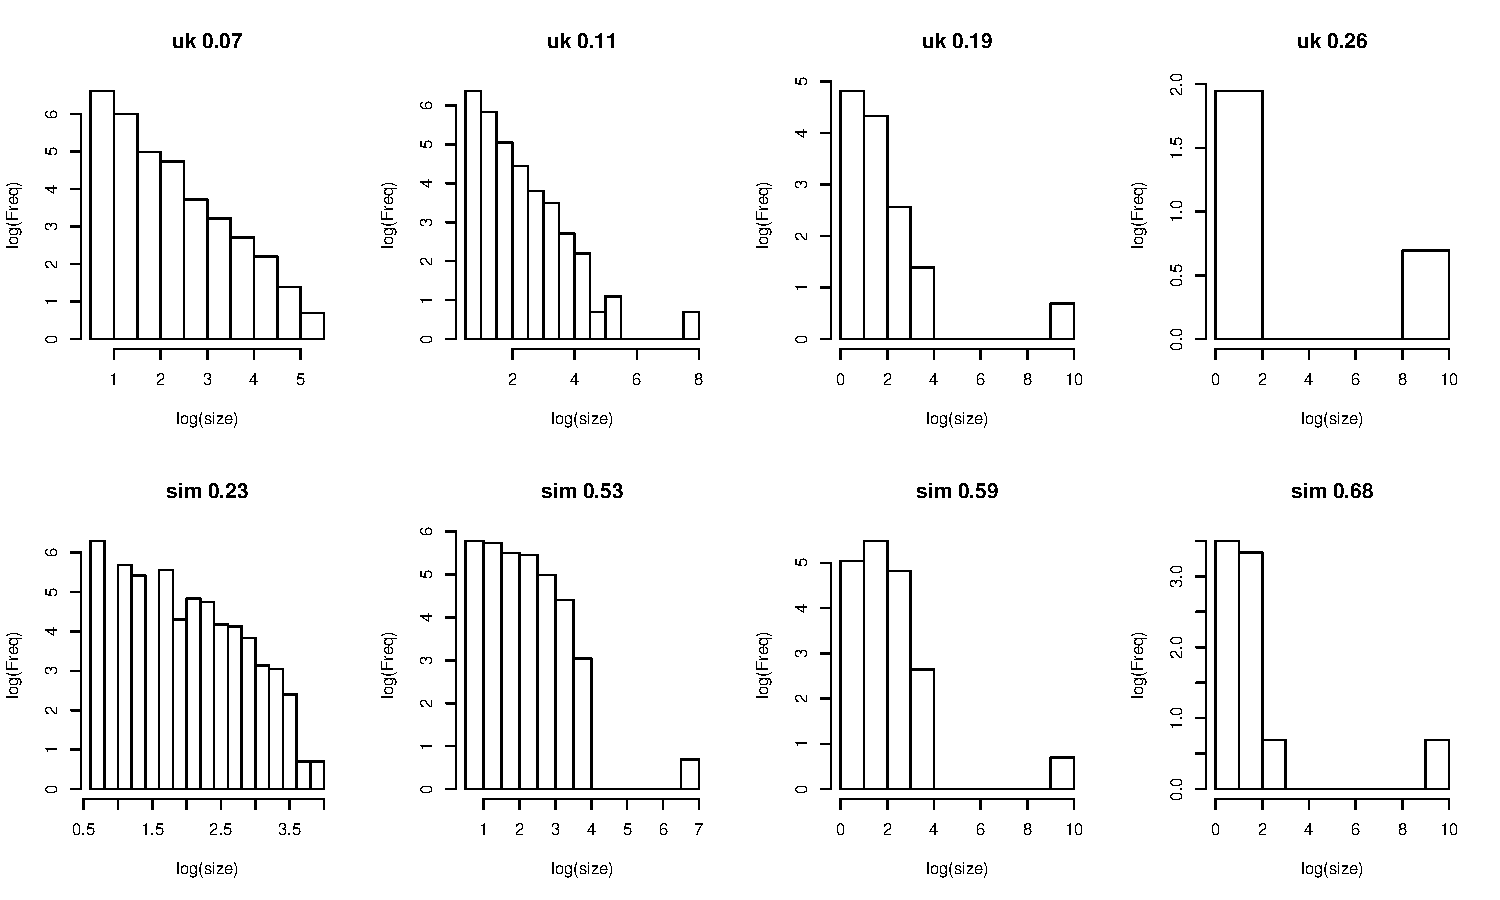
\includegraphics[width=10cm]{figure/plotplot_log-log-1} 

}



\end{knitrout}

QQ plots UK vs simulated, untransformed and log-log
\begin{knitrout}
\definecolor{shadecolor}{rgb}{0.969, 0.969, 0.969}\color{fgcolor}\begin{kframe}
\begin{alltt}
\hlkwd{par}\hlstd{(}\hlkwc{mfcol}\hlstd{=}\hlkwd{c}\hlstd{(}\hlnum{2}\hlstd{,} \hlkwd{max}\hlstd{(a, b)))}
\hlkwa{for} \hlstd{(i} \hlkwa{in} \hlnum{1}\hlopt{:}\hlkwd{max}\hlstd{(a, b))\{}
  \hlkwd{qqplot}\hlstd{(ukfreqClust[[i]]}\hlopt{$}\hlstd{Freq,}
         \hlstd{simfreqClust[[i]]}\hlopt{$}\hlstd{Freq,}
         \hlkwc{main} \hlstd{=} \hlkwd{paste}\hlstd{(}\hlstr{"uk:"}\hlstd{,} \hlkwd{names}\hlstd{(ukfreqClust)[i],}
                      \hlstr{"sim:"}\hlstd{,} \hlkwd{names}\hlstd{(simfreqClust)[i]),}
         \hlkwc{xlab} \hlstd{=} \hlstr{"uk"}\hlstd{,} \hlkwc{ylab} \hlstd{=} \hlstr{"sim"}\hlstd{)}

  \hlkwd{qqplot}\hlstd{(}\hlkwd{log}\hlstd{(ukfreqClust[[i]]}\hlopt{$}\hlstd{Freq),}
         \hlkwd{log}\hlstd{(simfreqClust[[i]]}\hlopt{$}\hlstd{Freq),}
         \hlkwc{main} \hlstd{=} \hlkwd{paste}\hlstd{(}\hlstr{"uk:"}\hlstd{,} \hlkwd{names}\hlstd{(ukfreqClust)[i],}
                      \hlstr{"sim:"}\hlstd{,} \hlkwd{names}\hlstd{(simfreqClust)[i]),}
         \hlkwc{xlab} \hlstd{=} \hlstr{"log(uk)"}\hlstd{,} \hlkwc{ylab} \hlstd{=} \hlstr{"log(sim)"}\hlstd{)}

\hlstd{\}}
\hlkwd{dev.off}\hlstd{()}
\end{alltt}
\begin{verbatim}
null device 
          1 
\end{verbatim}
\end{kframe}

{\centering 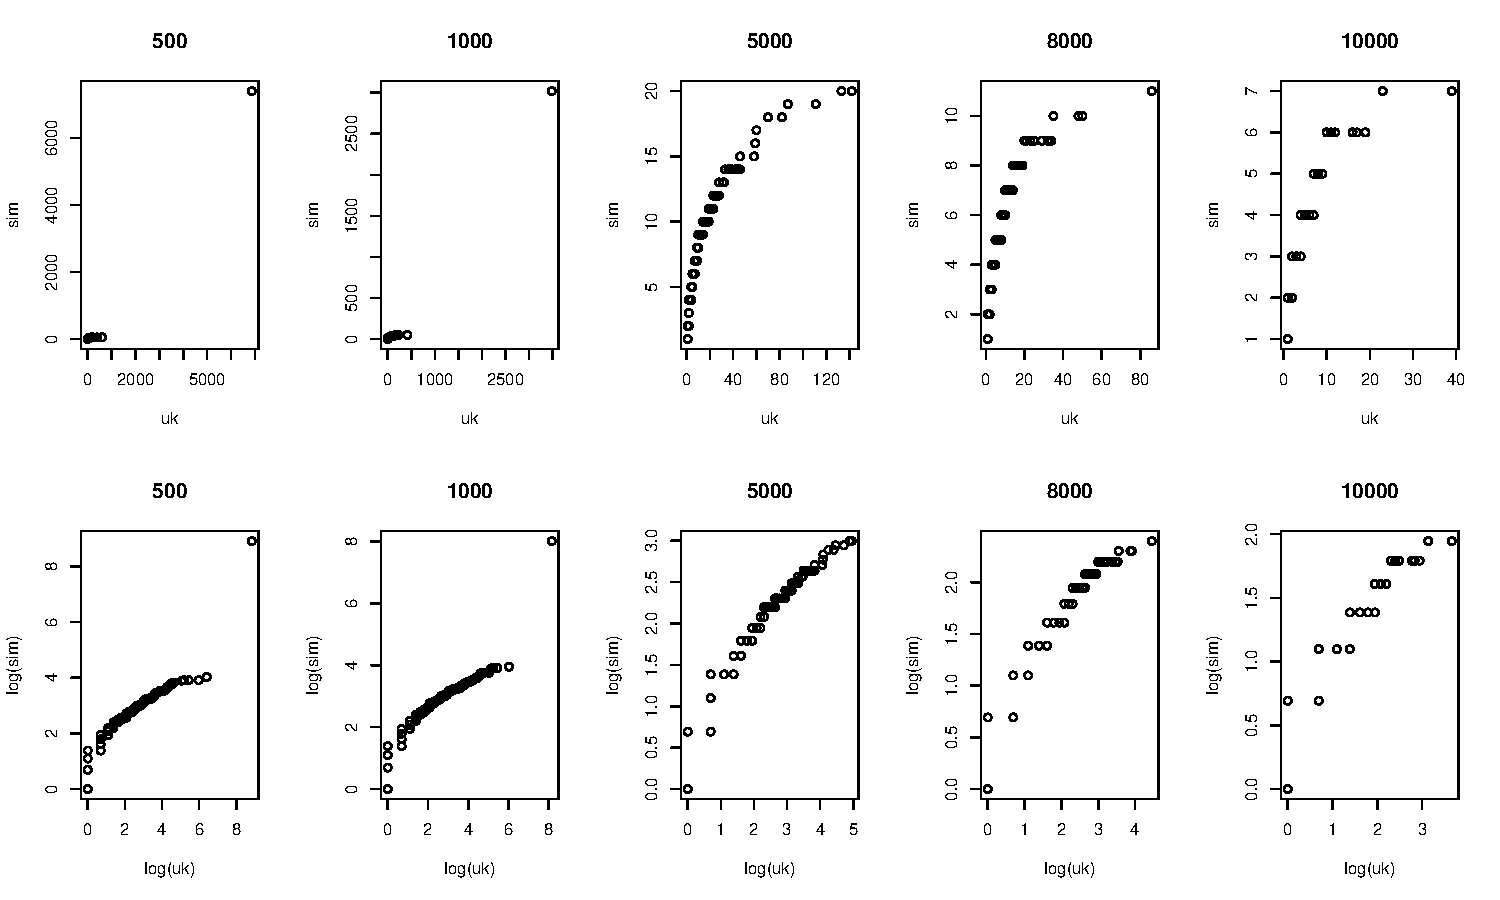
\includegraphics[width=10cm]{figure/plotQQ_plot-1} 

}



\end{knitrout}

\section{Associations}
After merging with co-variates allocated from demes states contained in tree, non-clustering individuals are assigned a cluster size of 1. 
\begin{knitrout}
\definecolor{shadecolor}{rgb}{0.969, 0.969, 0.969}\color{fgcolor}\begin{kframe}
\begin{alltt}
\hlcom{##- converting sample states in table of co-variates ?}

\hlkwa{if}\hlstd{(}\hlnum{TRUE}\hlstd{)\{}
\hlcom{# sampleTimes <- tree$sampleTimes}
\hlcom{# sampleStates  <- tree$sampleStates }

\hlstd{demo} \hlkwb{<-} \hlkwd{matrix}\hlstd{(}\hlnum{NA}\hlstd{,} \hlkwc{nrow} \hlstd{=}  \hlkwd{length}\hlstd{(tree}\hlopt{$}\hlstd{sampleTimes),} \hlkwc{ncol} \hlstd{=} \hlnum{6}\hlstd{)}
\hlkwa{for} \hlstd{(i} \hlkwa{in} \hlnum{1}\hlopt{:}\hlkwd{dim}\hlstd{(sampleStates)[}\hlnum{1}\hlstd{])\{} \hlcom{# dim(ss)[1]}
  \hlstd{deme} \hlkwb{<-} \hlkwd{names}\hlstd{(}\hlkwd{which.max}\hlstd{(sampleStates[i,]))} \hlcom{# name of column which has max value}
  \hlstd{patient} \hlkwb{<-} \hlkwd{as.numeric}\hlstd{(}\hlkwd{rownames}\hlstd{(tree}\hlopt{$}\hlstd{sampleStates)[i])}
  \hlstd{time} \hlkwb{<-} \hlstd{sampleTimes[i]}
  \hlstd{age} \hlkwb{<-} \hlkwd{as.numeric}\hlstd{(} \hlkwd{regmatches}\hlstd{( deme,}
                \hlkwd{regexec}\hlstd{(} \hlstr{"\textbackslash{}\textbackslash{}.age([0-9])"}\hlstd{, deme) )[[}\hlnum{1}\hlstd{]][}\hlnum{2}\hlstd{] )}
  \hlstd{care} \hlkwb{<-} \hlkwd{as.numeric}\hlstd{(} \hlkwd{regmatches}\hlstd{( deme,}
                \hlkwd{regexec}\hlstd{(} \hlstr{"care([0-9])"}\hlstd{, deme) )[[}\hlnum{1}\hlstd{]][}\hlnum{2}\hlstd{] )}
  \hlstd{stage} \hlkwb{<-} \hlkwd{as.numeric}\hlstd{(} \hlkwd{regmatches}\hlstd{( deme,}
                \hlkwd{regexec}\hlstd{(} \hlstr{"stage([0-9])"}\hlstd{, deme) )[[}\hlnum{1}\hlstd{]][}\hlnum{2}\hlstd{] )}
  \hlstd{risk} \hlkwb{<-} \hlkwd{as.numeric}\hlstd{(} \hlkwd{regmatches}\hlstd{( deme,}
                \hlkwd{regexec}\hlstd{(} \hlstr{"riskLevel([0-9])"}\hlstd{, deme) )[[}\hlnum{1}\hlstd{]][}\hlnum{2}\hlstd{] )}
  \hlstd{demo[i,]} \hlkwb{<-} \hlkwd{cbind}\hlstd{(patient, time, age, care, stage, risk)}
\hlstd{\}}
\hlkwd{colnames}\hlstd{(demo)} \hlkwb{<-} \hlkwd{cbind}\hlstd{(}\hlstr{"patient"}\hlstd{,} \hlstr{"time"}\hlstd{,}
                        \hlstr{"age"}\hlstd{,} \hlstr{"care"}\hlstd{,} \hlstr{"stage"}\hlstd{,} \hlstr{"risk"}\hlstd{)}

\hlkwd{saveRDS}\hlstd{(}\hlkwd{as.data.frame}\hlstd{(demo),} \hlkwc{file} \hlstd{=} \hlstr{"demo.rds"}\hlstd{)}
\hlstd{\}}
\end{alltt}


{\ttfamily\noindent\bfseries\color{errorcolor}{Error in matrix(NA, nrow = length(tree\$sampleTimes), ncol = 6): object 'tree' not found}}\end{kframe}
\end{knitrout}

The proportion of individuals into clusters and stats for "size of cluster for each individuals"


\begin{knitrout}
\definecolor{shadecolor}{rgb}{0.969, 0.969, 0.969}\color{fgcolor}\begin{kframe}
\begin{alltt}
\hlcom{##-proportion in or out clusters}
\hlkwd{sapply}\hlstd{(l,} \hlkwa{function}\hlstd{(}\hlkwc{x}\hlstd{)} \hlkwd{round}\hlstd{(}\hlkwd{prop.table}\hlstd{(}\hlkwd{table}\hlstd{(x}\hlopt{$}\hlstd{binclus)),}\hlnum{2}\hlstd{))}
\end{alltt}
\begin{verbatim}
  0.23 0.53 0.59 0.68
0  0.1 0.04 0.02 0.01
1  0.9 0.96 0.98 0.99
\end{verbatim}
\begin{alltt}
\hlcom{##- cluster sizes (by individuals having such a size !!)}
\hlkwd{sapply}\hlstd{(l,} \hlkwa{function}\hlstd{(}\hlkwc{x}\hlstd{)} \hlkwd{summary}\hlstd{(x}\hlopt{$}\hlstd{size))}
\end{alltt}
\begin{verbatim}
          0.23   0.53 0.59  0.68
Min.     1.000   1.00    1     1
1st Qu.  3.000   6.00   20 11900
Median   8.000  13.00 8766 11900
Mean     9.889  93.94 6320 11640
3rd Qu. 14.000  25.00 8766 11900
Max.    47.000 989.00 8766 11900
\end{verbatim}
\end{kframe}
\end{knitrout}



\section{Naive regressions on simulation}

Linear
\begin{knitrout}
\definecolor{shadecolor}{rgb}{0.969, 0.969, 0.969}\color{fgcolor}\begin{kframe}
\begin{alltt}
\hlcom{###### just on low and high threshold}
\hlstd{simli} \hlkwb{<-} \hlstd{listclus[}\hlkwd{c}\hlstd{(}\hlnum{1}\hlopt{:}\hlkwd{length}\hlstd{(listclus))]}

\hlstd{lm_model_std} \hlkwb{=} \hlstr{"scale(size) ~ scale(age) + scale(stage) + scale(time) + scale(risk)"}
\hlkwd{lapply}\hlstd{(simli ,} \hlkwa{function}\hlstd{(}\hlkwc{x}\hlstd{)} \hlkwd{summary}\hlstd{(}\hlkwd{lm}\hlstd{(lm_model_std,} \hlkwc{data} \hlstd{= x)))}
\end{alltt}
\begin{verbatim}
$`0.23`

Call:
lm(formula = lm_model_std, data = x)

Residuals:
    Min      1Q  Median      3Q     Max 
-1.5786 -0.6667 -0.2748  0.4126  5.0163 

Coefficients:
               Estimate Std. Error t value Pr(>|t|)    
(Intercept)  -9.297e-16  8.715e-03   0.000  1.00000    
scale(age)   -1.061e-02  8.783e-03  -1.208  0.22695    
scale(stage) -2.794e-02  8.788e-03  -3.180  0.00148 ** 
scale(time)   2.711e-01  8.749e-03  30.988  < 2e-16 ***
scale(risk)  -2.295e-02  8.717e-03  -2.633  0.00848 ** 
---
Signif. codes:  0 '***' 0.001 '**' 0.01 '*' 0.05 '.' 0.1 ' ' 1

Residual standard error: 0.9612 on 12159 degrees of freedom
Multiple R-squared:  0.07647,	Adjusted R-squared:  0.07616 
F-statistic: 251.7 on 4 and 12159 DF,  p-value: < 2.2e-16


$`0.53`

Call:
lm(formula = lm_model_std, data = x)

Residuals:
    Min      1Q  Median      3Q     Max 
-0.5101 -0.3449 -0.2843 -0.2215  3.4788 

Coefficients:
               Estimate Std. Error t value Pr(>|t|)    
(Intercept)   5.133e-15  9.050e-03   0.000    1.000    
scale(age)   -5.690e-03  9.121e-03  -0.624    0.533    
scale(stage) -5.758e-03  9.127e-03  -0.631    0.528    
scale(time)  -6.303e-02  9.086e-03  -6.937  4.2e-12 ***
scale(risk)   5.542e-03  9.052e-03   0.612    0.540    
---
Signif. codes:  0 '***' 0.001 '**' 0.01 '*' 0.05 '.' 0.1 ' ' 1

Residual standard error: 0.9982 on 12159 degrees of freedom
Multiple R-squared:  0.003982,	Adjusted R-squared:  0.003655 
F-statistic: 12.15 on 4 and 12159 DF,  p-value: 7.344e-10


$`0.59`

Call:
lm(formula = lm_model_std, data = x)

Residuals:
    Min      1Q  Median      3Q     Max 
-1.8811 -1.3122  0.4819  0.7101  1.0111 

Coefficients:
               Estimate Std. Error t value Pr(>|t|)    
(Intercept)   6.091e-14  8.851e-03   0.000    1.000    
scale(age)   -3.231e-03  8.920e-03  -0.362    0.717    
scale(stage) -5.990e-03  8.925e-03  -0.671    0.502    
scale(time)  -2.184e-01  8.886e-03 -24.575   <2e-16 ***
scale(risk)  -1.773e-03  8.853e-03  -0.200    0.841    
---
Signif. codes:  0 '***' 0.001 '**' 0.01 '*' 0.05 '.' 0.1 ' ' 1

Residual standard error: 0.9761 on 12159 degrees of freedom
Multiple R-squared:  0.04746,	Adjusted R-squared:  0.04715 
F-statistic: 151.5 on 4 and 12159 DF,  p-value: < 2.2e-16


$`0.68`

Call:
lm(formula = lm_model_std, data = x)

Residuals:
    Min      1Q  Median      3Q     Max 
-6.7106  0.0242  0.1557  0.2667  0.4853 

Coefficients:
               Estimate Std. Error t value Pr(>|t|)    
(Intercept)   2.957e-14  8.948e-03   0.000   1.0000    
scale(age)    2.061e-02  9.018e-03   2.286   0.0223 *  
scale(stage)  1.577e-02  9.024e-03   1.748   0.0806 .  
scale(time)  -1.574e-01  8.984e-03 -17.525   <2e-16 ***
scale(risk)   2.760e-03  8.951e-03   0.308   0.7578    
---
Signif. codes:  0 '***' 0.001 '**' 0.01 '*' 0.05 '.' 0.1 ' ' 1

Residual standard error: 0.9869 on 12159 degrees of freedom
Multiple R-squared:  0.02629,	Adjusted R-squared:  0.02597 
F-statistic: 82.07 on 4 and 12159 DF,  p-value: < 2.2e-16
\end{verbatim}
\end{kframe}
\end{knitrout}

Logistic
\begin{knitrout}
\definecolor{shadecolor}{rgb}{0.969, 0.969, 0.969}\color{fgcolor}\begin{kframe}
\begin{alltt}
\hlcom{##- model: clus ~ age +  stage + time + risk}
\hlcom{##- care = 1 for all at diagnosis}
\hlcom{## ex. }
\hlstd{logit_model_std} \hlkwb{=} \hlstr{"binclus ~ scale(age) + scale(stage) + scale(time) + scale(risk)"}
\hlkwd{lapply}\hlstd{(simli ,} \hlkwa{function}\hlstd{(}\hlkwc{x}\hlstd{)} \hlkwd{summary}\hlstd{(}\hlkwd{glm}\hlstd{(}\hlkwc{formula} \hlstd{= logit_model_std,}
                                   \hlkwc{data} \hlstd{= x,}
                                   \hlkwc{family} \hlstd{=} \hlkwd{binomial}\hlstd{(}\hlkwc{link} \hlstd{=} \hlstr{"logit"}\hlstd{))}
\hlstd{))}
\end{alltt}
\begin{verbatim}
$`0.23`

Call:
glm(formula = logit_model_std, family = binomial(link = "logit"), 
    data = x)

Deviance Residuals: 
    Min       1Q   Median       3Q      Max  
-3.0628   0.2197   0.3236   0.4602   1.2497  

Coefficients:
             Estimate Std. Error z value Pr(>|z|)    
(Intercept)   2.60860    0.04097  63.672  < 2e-16 ***
scale(age)   -0.09705    0.03496  -2.776   0.0055 ** 
scale(stage) -0.13678    0.03232  -4.232 2.31e-05 ***
scale(time)   0.98278    0.03314  29.660  < 2e-16 ***
scale(risk)  -0.14937    0.02985  -5.005 5.59e-07 ***
---
Signif. codes:  0 '***' 0.001 '**' 0.01 '*' 0.05 '.' 0.1 ' ' 1

(Dispersion parameter for binomial family taken to be 1)

    Null deviance: 7906.9  on 12163  degrees of freedom
Residual deviance: 6824.6  on 12159  degrees of freedom
AIC: 6834.6

Number of Fisher Scoring iterations: 6


$`0.53`

Call:
glm(formula = logit_model_std, family = binomial(link = "logit"), 
    data = x)

Deviance Residuals: 
    Min       1Q   Median       3Q      Max  
-3.1771   0.1841   0.2435   0.3244   0.7247  

Coefficients:
             Estimate Std. Error z value Pr(>|z|)    
(Intercept)   3.35884    0.05545  60.571  < 2e-16 ***
scale(age)   -0.11499    0.04934  -2.331  0.01978 *  
scale(stage) -0.12598    0.04521  -2.786  0.00533 ** 
scale(time)   0.74855    0.04452  16.812  < 2e-16 ***
scale(risk)  -0.09854    0.04205  -2.344  0.01909 *  
---
Signif. codes:  0 '***' 0.001 '**' 0.01 '*' 0.05 '.' 0.1 ' ' 1

(Dispersion parameter for binomial family taken to be 1)

    Null deviance: 4425.6  on 12163  degrees of freedom
Residual deviance: 4097.1  on 12159  degrees of freedom
AIC: 4107.1

Number of Fisher Scoring iterations: 6


$`0.59`

Call:
glm(formula = logit_model_std, family = binomial(link = "logit"), 
    data = x)

Deviance Residuals: 
    Min       1Q   Median       3Q      Max  
-2.9316   0.1921   0.2072   0.2231   0.2734  

Coefficients:
             Estimate Std. Error z value Pr(>|z|)    
(Intercept)   3.82076    0.06319  60.461  < 2e-16 ***
scale(age)   -0.05900    0.06416  -0.919  0.35784    
scale(stage) -0.16270    0.06298  -2.583  0.00978 ** 
scale(time)  -0.03569    0.06271  -0.569  0.56921    
scale(risk)  -0.09539    0.05813  -1.641  0.10079    
---
Signif. codes:  0 '***' 0.001 '**' 0.01 '*' 0.05 '.' 0.1 ' ' 1

(Dispersion parameter for binomial family taken to be 1)

    Null deviance: 2559.8  on 12163  degrees of freedom
Residual deviance: 2548.8  on 12159  degrees of freedom
AIC: 2558.8

Number of Fisher Scoring iterations: 6


$`0.68`

Call:
glm(formula = logit_model_std, family = binomial(link = "logit"), 
    data = x)

Deviance Residuals: 
    Min       1Q   Median       3Q      Max  
-3.4607   0.0303   0.0623   0.1195   0.3359  

Coefficients:
             Estimate Std. Error z value Pr(>|z|)    
(Intercept)   6.40088    0.27710  23.099   <2e-16 ***
scale(age)    0.03189    0.11270   0.283    0.777    
scale(stage) -0.14424    0.11961  -1.206    0.228    
scale(time)  -1.90394    0.23043  -8.262   <2e-16 ***
scale(risk)  -0.05687    0.11475  -0.496    0.620    
---
Signif. codes:  0 '***' 0.001 '**' 0.01 '*' 0.05 '.' 0.1 ' ' 1

(Dispersion parameter for binomial family taken to be 1)

    Null deviance: 871.97  on 12163  degrees of freedom
Residual deviance: 755.78  on 12159  degrees of freedom
AIC: 765.78

Number of Fisher Scoring iterations: 9
\end{verbatim}
\begin{alltt}
\hlcom{###--- sort dependency between indivduals from same cluster}
\hlcom{### 1. downsample to make analysis of one cluster size}
\hlcom{###  explained by median or mean of each co-variate.}
\hlcom{###  2. plot the distribution of covariates by cluster size. }
\hlcom{###  With the intuition that smaller clusters are more explained}
\hlcom{###  by covariates and larger ones are more random. }
\hlcom{###  Do it on real data and simulation}

\hlcom{# For each cluster size, compute mean of all coavariates}
\end{alltt}
\end{kframe}
\end{knitrout}

\section{Regressions on down-sampled simulation}
To sort out the dependency between individuals from same cluster
\begin{enumerate}
\item "downsample" to make analysis of each cluster size explained by mean of each co-variate (from here, only clusters from lower and higher threshold represented)

\begin{knitrout}
\definecolor{shadecolor}{rgb}{0.969, 0.969, 0.969}\color{fgcolor}\begin{kframe}
\begin{alltt}
\hlcom{##- 1. down-sample: mean of each variable}
\hlstd{down} \hlkwb{<-} \hlkwd{lapply}\hlstd{(simli,} \hlkwa{function}\hlstd{(}\hlkwc{x}\hlstd{)} \hlkwd{aggregate}\hlstd{(x[,} \hlnum{5}\hlopt{:}\hlnum{9}\hlstd{],} \hlkwd{list}\hlstd{(}\hlstr{"size"} \hlstd{= x}\hlopt{$}\hlstd{size), mean))}
\hlcom{# str(down)}

\hlcom{##- linear regression}
\hlkwd{lapply}\hlstd{(down,} \hlkwa{function}\hlstd{(}\hlkwc{x}\hlstd{)} \hlkwd{summary}\hlstd{(}\hlkwd{lm}\hlstd{(lm_model_std,} \hlkwc{data} \hlstd{= x)))}
\end{alltt}
\begin{verbatim}
$`0.23`

Call:
lm(formula = lm_model_std, data = x)

Residuals:
    Min      1Q  Median      3Q     Max 
-1.1082 -0.5070 -0.2067  0.4938  2.7281 

Coefficients:
               Estimate Std. Error t value Pr(>|t|)  
(Intercept)   3.337e-16  1.381e-01   0.000   1.0000  
scale(age)   -1.385e-01  1.582e-01  -0.876   0.3878  
scale(stage) -1.781e-01  1.684e-01  -1.058   0.2981  
scale(time)   4.213e-01  1.963e-01   2.146   0.0396 *
scale(risk)  -8.551e-02  1.744e-01  -0.490   0.6274  
---
Signif. codes:  0 '***' 0.001 '**' 0.01 '*' 0.05 '.' 0.1 ' ' 1

Residual standard error: 0.84 on 32 degrees of freedom
Multiple R-squared:  0.3728,	Adjusted R-squared:  0.2944 
F-statistic: 4.756 on 4 and 32 DF,  p-value: 0.003991


$`0.53`

Call:
lm(formula = lm_model_std, data = x)

Residuals:
    Min      1Q  Median      3Q     Max 
-0.7323 -0.2221 -0.1173 -0.0221  6.3887 

Coefficients:
               Estimate Std. Error t value Pr(>|t|)
(Intercept)  -1.039e-16  1.500e-01   0.000    1.000
scale(age)   -1.030e-01  1.737e-01  -0.593    0.556
scale(stage) -1.217e-01  1.909e-01  -0.637    0.527
scale(time)  -2.281e-01  1.897e-01  -1.202    0.236
scale(risk)   3.922e-02  1.640e-01   0.239    0.812

Residual standard error: 1.029 on 42 degrees of freedom
Multiple R-squared:  0.03415,	Adjusted R-squared:  -0.05783 
F-statistic: 0.3713 on 4 and 42 DF,  p-value: 0.8278


$`0.59`

Call:
lm(formula = lm_model_std, data = x)

Residuals:
    Min      1Q  Median      3Q     Max 
-1.0914 -0.4985 -0.0551  0.1814  3.7754 

Coefficients:
               Estimate Std. Error t value Pr(>|t|)   
(Intercept)  -9.422e-16  1.711e-01   0.000  1.00000   
scale(age)    1.214e-01  2.132e-01   0.570  0.57425   
scale(stage) -2.134e-01  2.051e-01  -1.040  0.30864   
scale(time)  -5.841e-01  1.967e-01  -2.970  0.00666 **
scale(risk)  -9.436e-02  2.090e-01  -0.451  0.65570   
---
Signif. codes:  0 '***' 0.001 '**' 0.01 '*' 0.05 '.' 0.1 ' ' 1

Residual standard error: 0.9215 on 24 degrees of freedom
Multiple R-squared:  0.2722,	Adjusted R-squared:  0.1509 
F-statistic: 2.244 on 4 and 24 DF,  p-value: 0.09424


$`0.68`

Call:
lm(formula = lm_model_std, data = x)

Residuals:
       1        2        3        4        5        6        7        8        9 
 0.16838 -0.22310  0.06874  0.24689  0.01718  0.08857 -0.29756 -0.16086  0.09177 
attr(,"scaled:center")
[1] 1327
attr(,"scaled:scale")
[1] 3965

Coefficients:
               Estimate Std. Error t value Pr(>|t|)    
(Intercept)  -7.721e-16  8.737e-02   0.000 1.000000    
scale(age)   -1.782e-01  2.319e-01  -0.768 0.485203    
scale(stage) -2.047e-02  1.971e-01  -0.104 0.922257    
scale(time)  -1.087e+00  1.181e-01  -9.206 0.000773 ***
scale(risk)   9.266e-03  1.305e-01   0.071 0.946805    
---
Signif. codes:  0 '***' 0.001 '**' 0.01 '*' 0.05 '.' 0.1 ' ' 1

Residual standard error: 0.2621 on 4 degrees of freedom
Multiple R-squared:  0.9657,	Adjusted R-squared:  0.9313 
F-statistic: 28.11 on 4 and 4 DF,  p-value: 0.003458
\end{verbatim}
\end{kframe}
\end{knitrout}


\item plot the distribution of covariates by cluster size

\begin{knitrout}
\definecolor{shadecolor}{rgb}{0.969, 0.969, 0.969}\color{fgcolor}\begin{kframe}
\begin{alltt}
\hlcom{##- 2. plots}
\hlkwd{library}\hlstd{(lattice)}
\hlcom{# trellis.par.set(canonical.theme(color = FALSE))}
\hlkwa{for}\hlstd{(i} \hlkwa{in} \hlnum{1}\hlopt{:}\hlkwd{length}\hlstd{(simli))\{}
  \hlkwd{print}\hlstd{(}\hlkwd{histogram}\hlstd{(}\hlopt{~} \hlstd{stage}\hlopt{|}\hlkwd{factor}\hlstd{(size),}
            \hlkwc{main} \hlstd{=} \hlkwd{paste}\hlstd{(}\hlstr{"distribution of stages by cluster sizes at threshold ="}\hlstd{,} \hlkwd{names}\hlstd{(simli[i])),}
            \hlkwc{data} \hlstd{= simli[[i]])}
  \hlstd{)}
\hlstd{\}}
\end{alltt}
\end{kframe}

{\centering 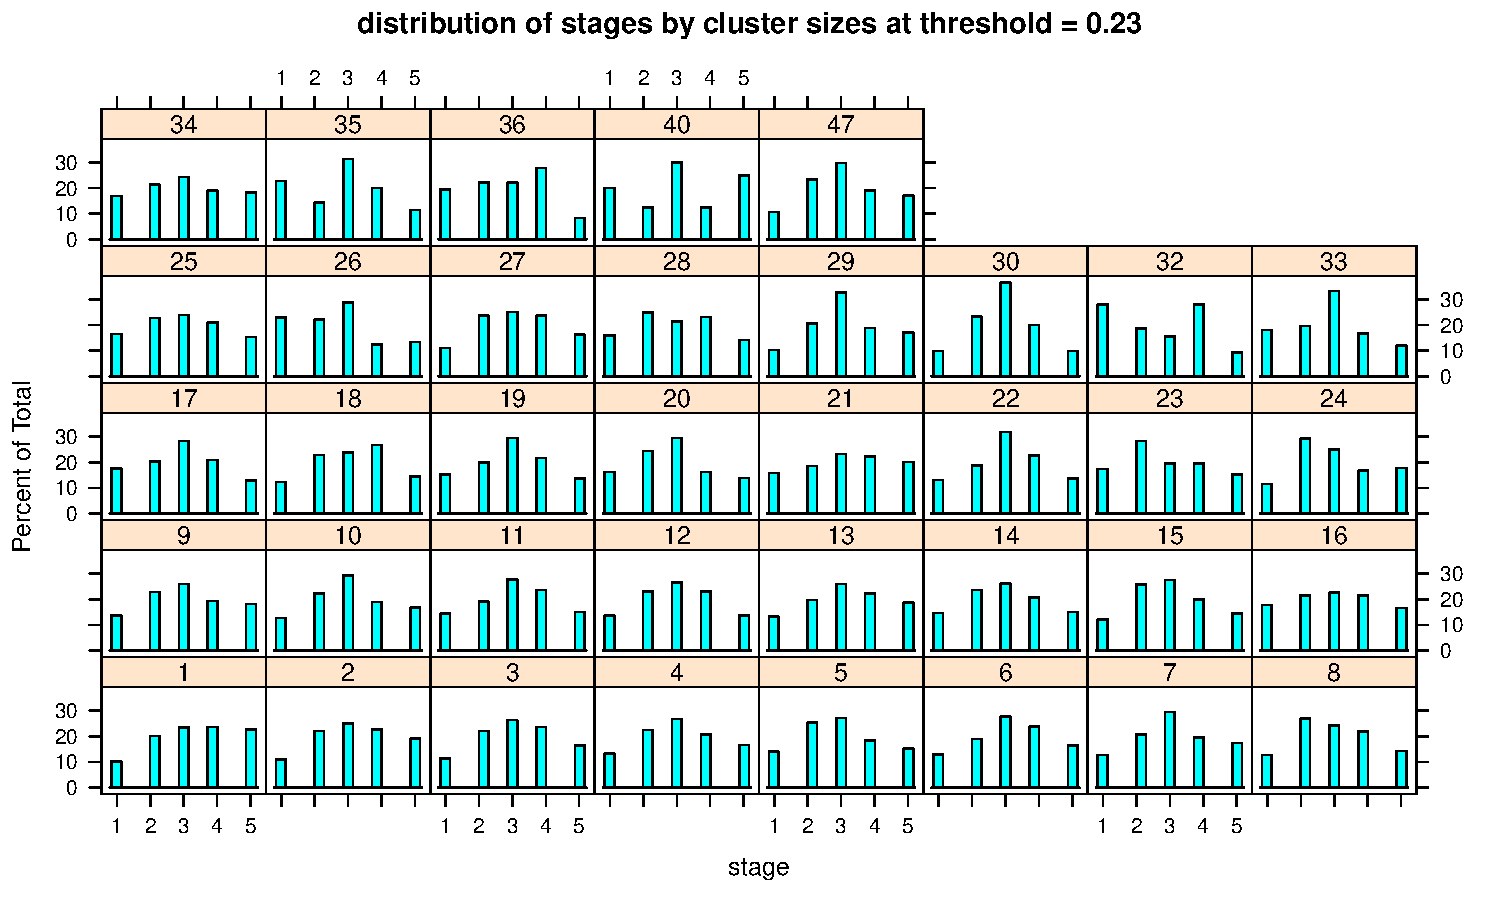
\includegraphics[width=10cm]{figure/plotlattice-1} 
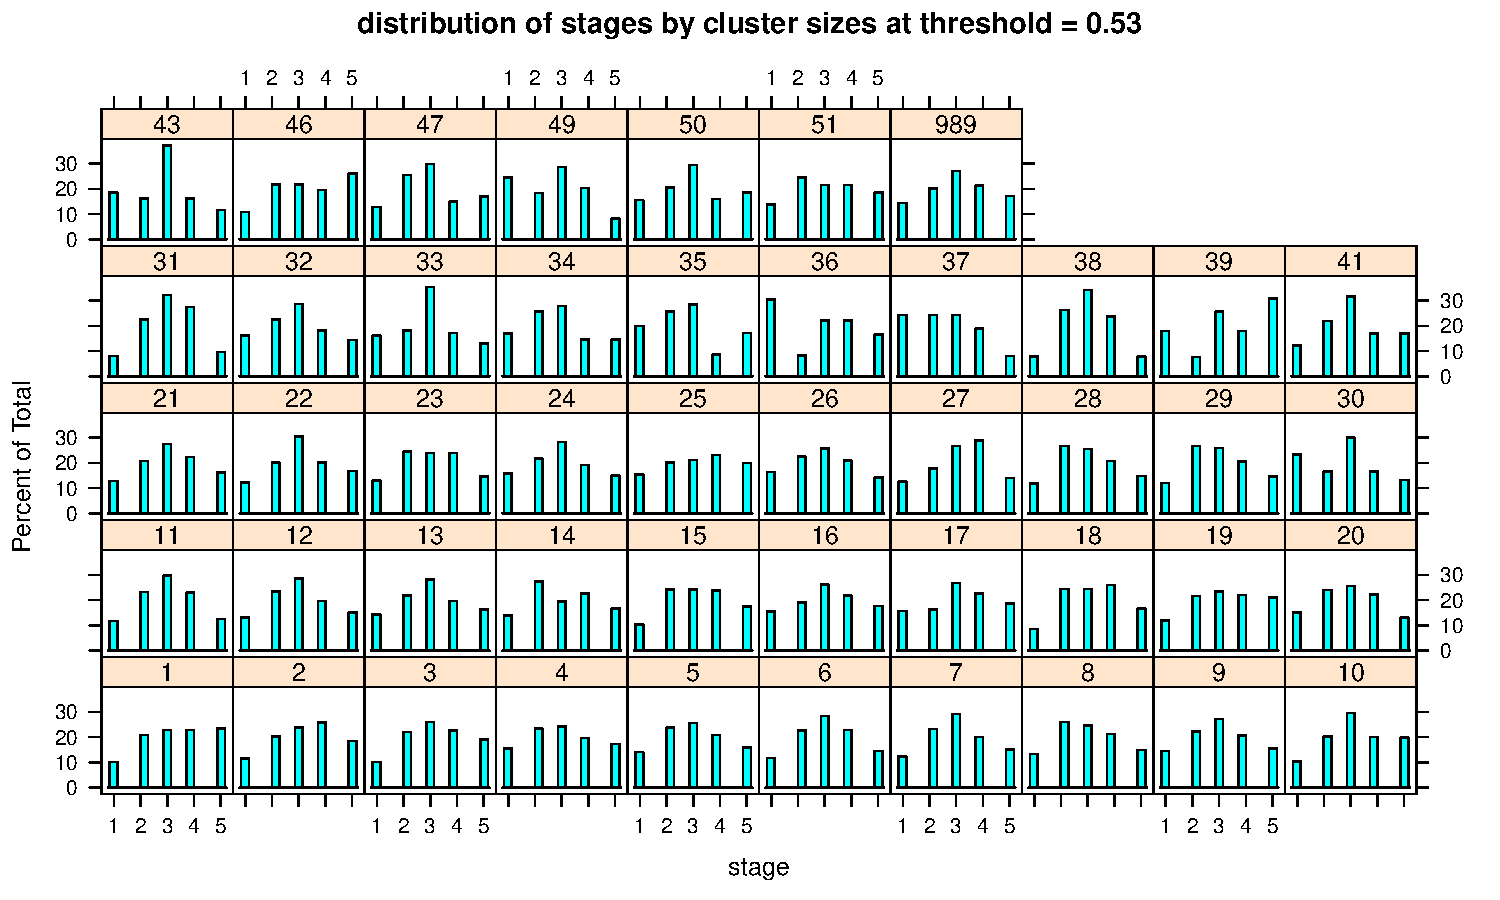
\includegraphics[width=10cm]{figure/plotlattice-2} 
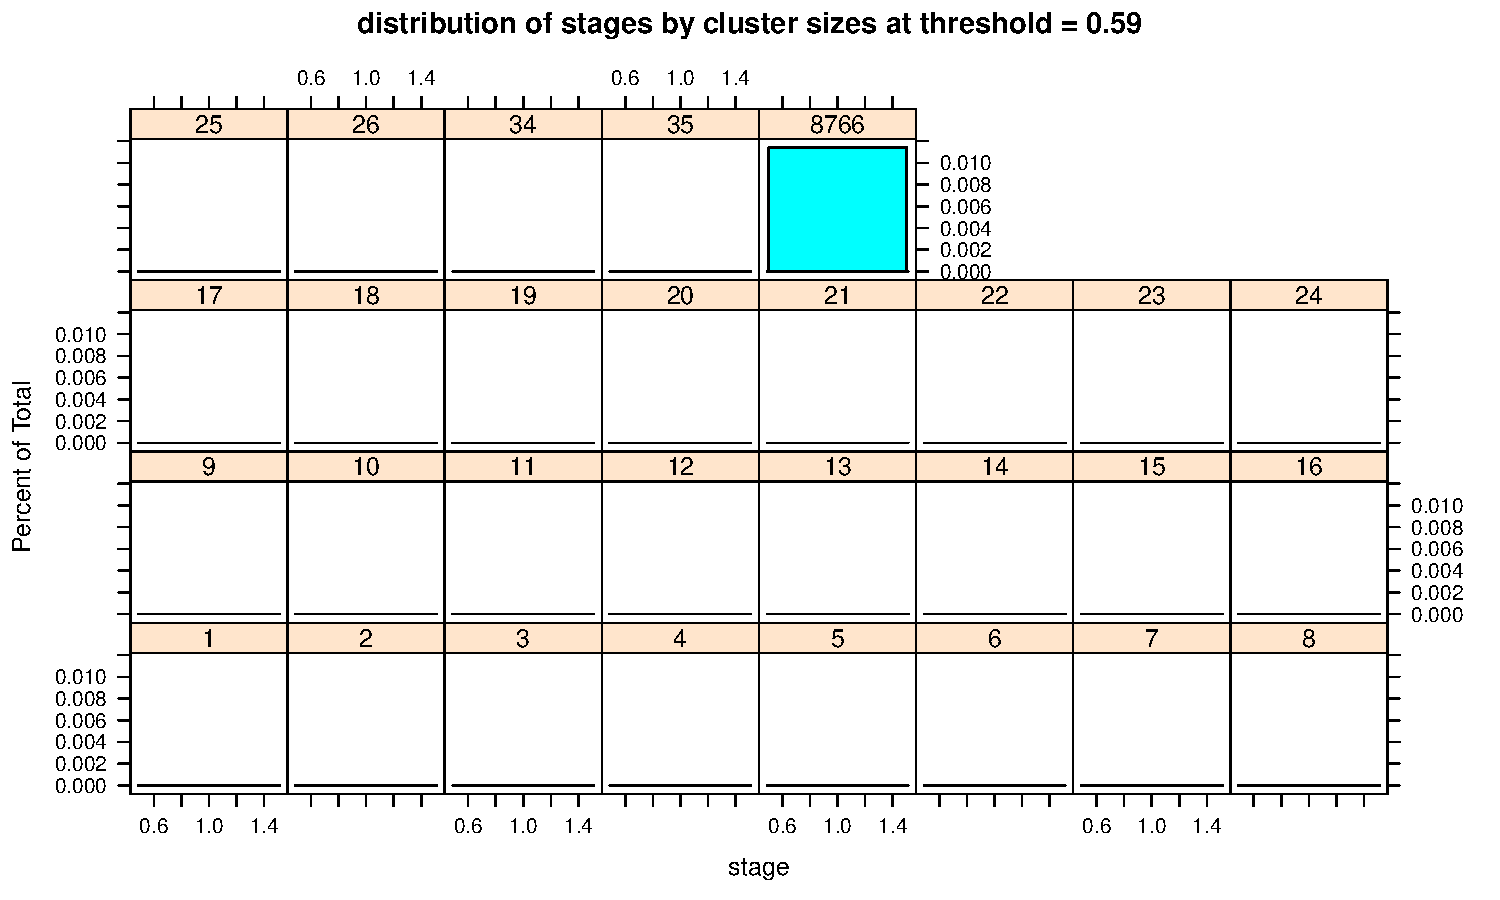
\includegraphics[width=10cm]{figure/plotlattice-3} 
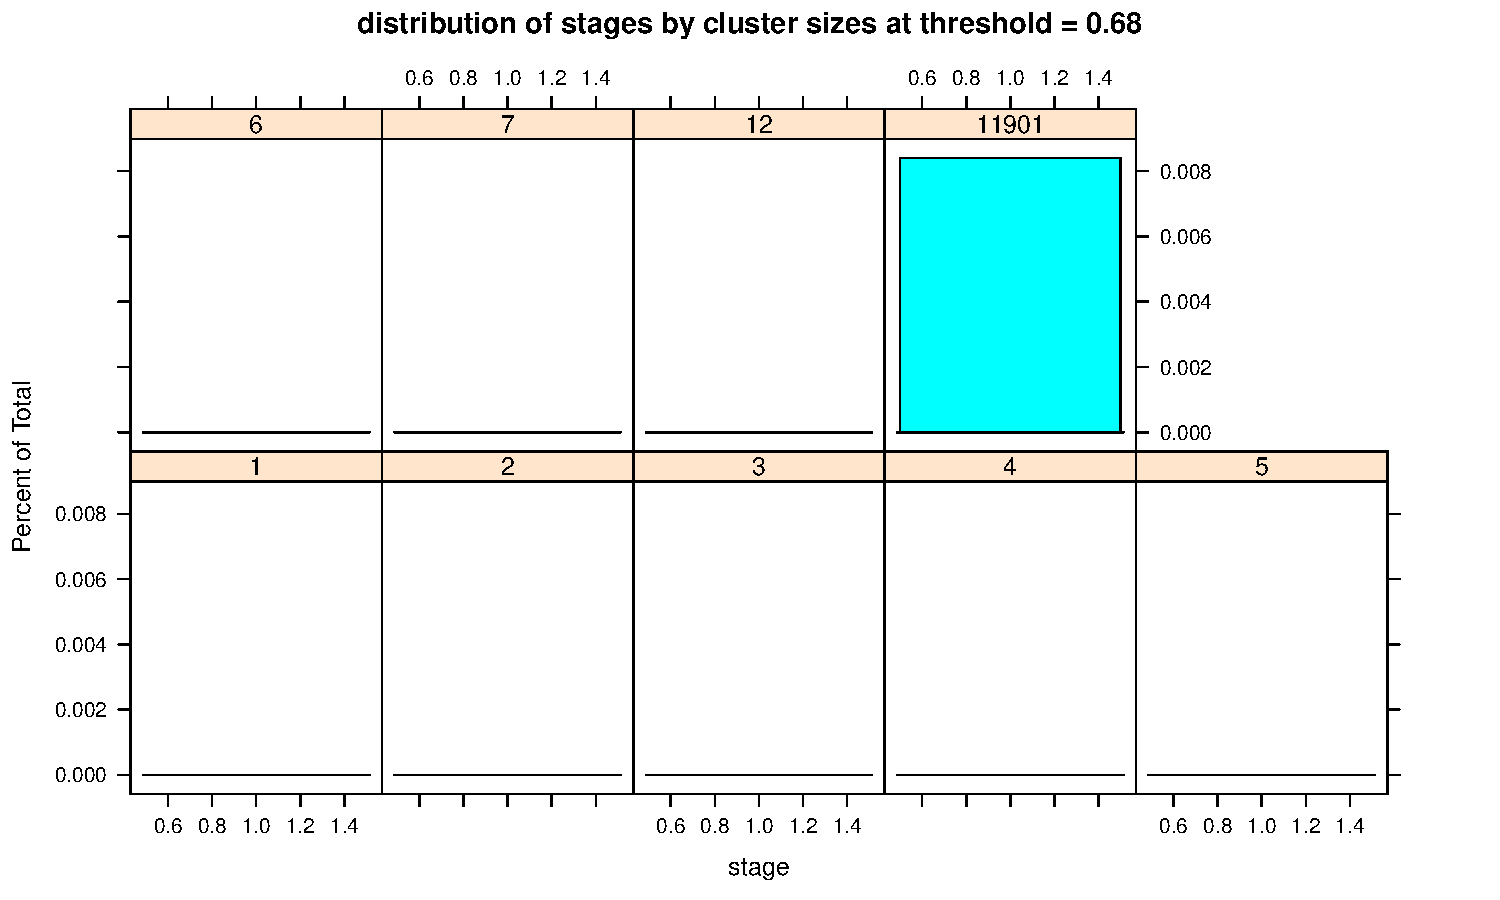
\includegraphics[width=10cm]{figure/plotlattice-4} 

}



\end{knitrout}


\end{enumerate}

\section{On real UK data}
Same process ...


Proportion in and out clusters
\begin{knitrout}
\definecolor{shadecolor}{rgb}{0.969, 0.969, 0.969}\color{fgcolor}\begin{kframe}
\begin{alltt}
\hlcom{##-proportion in or out clusters}
\hlkwd{sapply}\hlstd{(l,} \hlkwa{function}\hlstd{(}\hlkwc{x}\hlstd{)} \hlkwd{round}\hlstd{(}\hlkwd{prop.table}\hlstd{(}\hlkwd{table}\hlstd{(x}\hlopt{$}\hlstd{binclus)),}\hlnum{2}\hlstd{))}
\end{alltt}
\begin{verbatim}
  0.07 0.11 0.19 0.26
0 0.37 0.23 0.04    0
1 0.63 0.77 0.96    1
\end{verbatim}
\begin{alltt}
\hlcom{##- cluster sizes (by individuals having such a size !!)}
\hlkwd{sapply}\hlstd{(l,} \hlkwa{function}\hlstd{(}\hlkwc{x}\hlstd{)} \hlkwd{summary}\hlstd{(x}\hlopt{$}\hlstd{size))}
\end{alltt}
\begin{verbatim}
          0.07   0.11  0.19  0.26
Min.      1.00    1.0     1     1
1st Qu.   1.00    2.0 10900 12110
Median    3.00    8.0 10900 12110
Mean     15.47  426.5  9762 12060
3rd Qu.  12.00   62.0 10900 12110
Max.    162.00 2235.0 10900 12110
\end{verbatim}
\end{kframe}
\end{knitrout}



Naive regressions
\begin{knitrout}
\definecolor{shadecolor}{rgb}{0.969, 0.969, 0.969}\color{fgcolor}\begin{kframe}
\begin{alltt}
\hlcom{#### just on low and high threshold (but not too high !)}
\hlstd{li} \hlkwb{<-} \hlstd{listUKclus[} \hlnum{1}\hlopt{:}\hlstd{(}\hlkwd{length}\hlstd{(listUKclus)}\hlopt{-}\hlnum{1}\hlstd{) ]}
\hlstd{lm_model_std} \hlkwb{=} \hlstr{"scale(size) ~ scale(agediag) + scale(sqrt(cd4)) +  scale(ydiag)"}
\hlkwd{lapply}\hlstd{(li,} \hlkwa{function}\hlstd{(}\hlkwc{x}\hlstd{)} \hlkwd{summary}\hlstd{(}\hlkwd{lm}\hlstd{(lm_model_std,} \hlkwc{data} \hlstd{= x)))}
\end{alltt}
\begin{verbatim}
$`0.07`

Call:
lm(formula = lm_model_std, data = x)

Residuals:
    Min      1Q  Median      3Q     Max 
-0.8338 -0.4714 -0.2992 -0.0755  4.9307 

Coefficients:
                  Estimate Std. Error t value Pr(>|t|)    
(Intercept)       0.003156   0.009105   0.347  0.72893    
scale(agediag)   -0.025564   0.009495  -2.692  0.00711 ** 
scale(sqrt(cd4))  0.048448   0.009239   5.244  1.6e-07 ***
scale(ydiag)      0.166237   0.009431  17.627  < 2e-16 ***
---
Signif. codes:  0 '***' 0.001 '**' 0.01 '*' 0.05 '.' 0.1 ' ' 1

Residual standard error: 0.9916 on 11857 degrees of freedom
  (303 observations deleted due to missingness)
Multiple R-squared:  0.02869,	Adjusted R-squared:  0.02844 
F-statistic: 116.7 on 3 and 11857 DF,  p-value: < 2.2e-16


$`0.11`

Call:
lm(formula = lm_model_std, data = x)

Residuals:
    Min      1Q  Median      3Q     Max 
-1.1701 -0.5395 -0.3606 -0.1872  2.5272 

Coefficients:
                   Estimate Std. Error t value Pr(>|t|)    
(Intercept)       0.0001816  0.0089649   0.020   0.9838    
scale(agediag)    0.0757349  0.0093484   8.101 5.97e-16 ***
scale(sqrt(cd4))  0.0165371  0.0090965   1.818   0.0691 .  
scale(ydiag)     -0.2140942  0.0092853 -23.057  < 2e-16 ***
---
Signif. codes:  0 '***' 0.001 '**' 0.01 '*' 0.05 '.' 0.1 ' ' 1

Residual standard error: 0.9763 on 11857 degrees of freedom
  (303 observations deleted due to missingness)
Multiple R-squared:  0.04349,	Adjusted R-squared:  0.04324 
F-statistic: 179.7 on 3 and 11857 DF,  p-value: < 2.2e-16


$`0.19`

Call:
lm(formula = lm_model_std, data = x)

Residuals:
    Min      1Q  Median      3Q     Max 
-3.5153  0.1284  0.3212  0.4572  0.7435 

Coefficients:
                   Estimate Std. Error t value Pr(>|t|)    
(Intercept)       7.343e-04  9.030e-03   0.081    0.935    
scale(agediag)    8.434e-02  9.416e-03   8.956   <2e-16 ***
scale(sqrt(cd4)) -7.202e-06  9.162e-03  -0.001    0.999    
scale(ydiag)     -1.932e-01  9.353e-03 -20.661   <2e-16 ***
---
Signif. codes:  0 '***' 0.001 '**' 0.01 '*' 0.05 '.' 0.1 ' ' 1

Residual standard error: 0.9834 on 11857 degrees of freedom
  (303 observations deleted due to missingness)
Multiple R-squared:  0.0364,	Adjusted R-squared:  0.03616 
F-statistic: 149.3 on 3 and 11857 DF,  p-value: < 2.2e-16
\end{verbatim}
\end{kframe}
\end{knitrout}

\begin{knitrout}
\definecolor{shadecolor}{rgb}{0.969, 0.969, 0.969}\color{fgcolor}\begin{kframe}
\begin{alltt}
\hlcom{##- model: clus ~ age +  stage + time + risk}
\hlcom{##- care = 1 for all at diagnosis}
\hlcom{## ex. }
\hlstd{logit_model_std} \hlkwb{=} \hlstr{"binclus ~ scale(agediag) + scale(sqrt(cd4)) + scale(ydiag)"}
\hlkwd{lapply}\hlstd{(li,} \hlkwa{function}\hlstd{(}\hlkwc{x}\hlstd{)} \hlkwd{summary}\hlstd{(}\hlkwd{glm}\hlstd{(}\hlkwc{formula} \hlstd{= logit_model_std,}
                                     \hlkwc{data} \hlstd{= x,}
                                     \hlkwc{family} \hlstd{=} \hlkwd{binomial}\hlstd{(}\hlkwc{link} \hlstd{=} \hlstr{"logit"}\hlstd{))}
                               \hlstd{))}
\end{alltt}
\begin{verbatim}
$`0.07`

Call:
glm(formula = logit_model_std, family = binomial(link = "logit"), 
    data = x)

Deviance Residuals: 
    Min       1Q   Median       3Q      Max  
-2.2101  -1.0772   0.6772   0.8944   2.0267  

Coefficients:
                 Estimate Std. Error z value Pr(>|z|)    
(Intercept)       0.58725    0.02050  28.646  < 2e-16 ***
scale(agediag)   -0.14644    0.02125  -6.892 5.49e-12 ***
scale(sqrt(cd4))  0.26123    0.02067  12.640  < 2e-16 ***
scale(ydiag)      0.74823    0.02197  34.057  < 2e-16 ***
---
Signif. codes:  0 '***' 0.001 '**' 0.01 '*' 0.05 '.' 0.1 ' ' 1

(Dispersion parameter for binomial family taken to be 1)

    Null deviance: 15620  on 11860  degrees of freedom
Residual deviance: 14116  on 11857  degrees of freedom
  (303 observations deleted due to missingness)
AIC: 14124

Number of Fisher Scoring iterations: 4


$`0.11`

Call:
glm(formula = logit_model_std, family = binomial(link = "logit"), 
    data = x)

Deviance Residuals: 
    Min       1Q   Median       3Q      Max  
-2.2923   0.4860   0.6171   0.7352   1.3728  

Coefficients:
                 Estimate Std. Error z value Pr(>|z|)    
(Intercept)       1.27858    0.02301  55.560   <2e-16 ***
scale(agediag)   -0.04952    0.02343  -2.114   0.0345 *  
scale(sqrt(cd4))  0.23453    0.02248  10.433   <2e-16 ***
scale(ydiag)      0.43899    0.02247  19.540   <2e-16 ***
---
Signif. codes:  0 '***' 0.001 '**' 0.01 '*' 0.05 '.' 0.1 ' ' 1

(Dispersion parameter for binomial family taken to be 1)

    Null deviance: 12734  on 11860  degrees of freedom
Residual deviance: 12217  on 11857  degrees of freedom
  (303 observations deleted due to missingness)
AIC: 12225

Number of Fisher Scoring iterations: 4


$`0.19`

Call:
glm(formula = logit_model_std, family = binomial(link = "logit"), 
    data = x)

Deviance Residuals: 
    Min       1Q   Median       3Q      Max  
-2.9359   0.2445   0.2847   0.3260   0.4972  

Coefficients:
                 Estimate Std. Error z value Pr(>|z|)    
(Intercept)       3.18233    0.04862  65.451  < 2e-16 ***
scale(agediag)    0.22531    0.04997   4.509 6.52e-06 ***
scale(sqrt(cd4))  0.16324    0.04603   3.546 0.000391 ***
scale(ydiag)     -0.36144    0.05234  -6.906 4.98e-12 ***
---
Signif. codes:  0 '***' 0.001 '**' 0.01 '*' 0.05 '.' 0.1 ' ' 1

(Dispersion parameter for binomial family taken to be 1)

    Null deviance: 4182.4  on 11860  degrees of freedom
Residual deviance: 4114.1  on 11857  degrees of freedom
  (303 observations deleted due to missingness)
AIC: 4122.1

Number of Fisher Scoring iterations: 6
\end{verbatim}
\end{kframe}
\end{knitrout}

Down-sampled regressions
\begin{knitrout}
\definecolor{shadecolor}{rgb}{0.969, 0.969, 0.969}\color{fgcolor}\begin{kframe}
\begin{alltt}
\hlcom{##- 1. down-sample: MEDIAN of each variable (with na.rm = T)}

\hlcom{# head(li[[1]][, c("agediag", "sqrtcd4", "ydiag")])}
\hlstd{down_median} \hlkwb{<-} \hlkwd{lapply}\hlstd{(li,} \hlkwa{function}\hlstd{(}\hlkwc{x}\hlstd{)}
  \hlkwd{aggregate}\hlstd{(x[,} \hlkwd{c}\hlstd{(}\hlstr{"agediag"}\hlstd{,} \hlstr{"sqrtcd4"}\hlstd{,} \hlstr{"ydiag"}\hlstd{,} \hlstr{"logvl"}\hlstd{)],}
            \hlkwd{list}\hlstd{(}\hlstr{"size"} \hlstd{= x}\hlopt{$}\hlstd{size),}
            \hlkwa{function}\hlstd{(}\hlkwc{x}\hlstd{)} \hlkwd{median}\hlstd{(x,} \hlkwc{na.rm} \hlstd{=} \hlnum{TRUE}\hlstd{)))}

\hlstd{down_mean} \hlkwb{<-} \hlkwd{lapply}\hlstd{(li,} \hlkwa{function}\hlstd{(}\hlkwc{x}\hlstd{)}
  \hlkwd{aggregate}\hlstd{(x[,} \hlkwd{c}\hlstd{(}\hlstr{"agediag"}\hlstd{,} \hlstr{"sqrtcd4"}\hlstd{,} \hlstr{"ydiag"}\hlstd{,} \hlstr{"logvl"}\hlstd{)],}
            \hlkwd{list}\hlstd{(}\hlstr{"size"} \hlstd{= x}\hlopt{$}\hlstd{size),}
            \hlkwa{function}\hlstd{(}\hlkwc{x}\hlstd{)} \hlkwd{mean}\hlstd{(x,} \hlkwc{na.rm} \hlstd{=} \hlnum{TRUE}\hlstd{)))}
\hlcom{# str(down_mean) }
\hlcom{##- linear regression}
\hlstd{lm_model_std} \hlkwb{=} \hlstr{"scale(size) ~ scale(agediag) + scale(sqrtcd4) + scale(ydiag)"}
\hlkwd{lapply}\hlstd{(down_median,} \hlkwa{function}\hlstd{(}\hlkwc{x}\hlstd{)} \hlkwd{summary}\hlstd{(}\hlkwd{lm}\hlstd{(lm_model_std,} \hlkwc{data} \hlstd{= x)))}
\end{alltt}
\begin{verbatim}
$`0.07`

Call:
lm(formula = lm_model_std, data = x)

Residuals:
    Min      1Q  Median      3Q     Max 
-0.9520 -0.6592 -0.3118  0.3229  3.5106 

Coefficients:
                Estimate Std. Error t value Pr(>|t|)
(Intercept)    9.131e-16  1.439e-01   0.000    1.000
scale(agediag) 9.038e-02  1.663e-01   0.544    0.589
scale(sqrtcd4) 6.494e-02  1.683e-01   0.386    0.701
scale(ydiag)   2.181e-02  1.480e-01   0.147    0.883

Residual standard error: 1.028 on 47 degrees of freedom
Multiple R-squared:  0.007271,	Adjusted R-squared:  -0.05609 
F-statistic: 0.1148 on 3 and 47 DF,  p-value: 0.951


$`0.11`

Call:
lm(formula = lm_model_std, data = x)

Residuals:
    Min      1Q  Median      3Q     Max 
-1.0671 -0.3240 -0.1322  0.1768  6.1780 

Coefficients:
                 Estimate Std. Error t value Pr(>|t|)  
(Intercept)     2.836e-15  1.347e-01   0.000   1.0000  
scale(agediag) -3.660e-02  1.398e-01  -0.262   0.7946  
scale(sqrtcd4)  5.980e-02  1.440e-01   0.415   0.6797  
scale(ydiag)   -3.553e-01  1.469e-01  -2.418   0.0194 *
---
Signif. codes:  0 '***' 0.001 '**' 0.01 '*' 0.05 '.' 0.1 ' ' 1

Residual standard error: 0.9714 on 48 degrees of freedom
Multiple R-squared:  0.1119,	Adjusted R-squared:  0.05639 
F-statistic: 2.016 on 3 and 48 DF,  p-value: 0.1242


$`0.19`

Call:
lm(formula = lm_model_std, data = x)

Residuals:
     Min       1Q   Median       3Q      Max 
-1.31673 -0.43625  0.00839  0.08538  2.67861 

Coefficients:
                 Estimate Std. Error t value Pr(>|t|)  
(Intercept)     3.119e-14  2.123e-01   0.000   1.0000  
scale(agediag) -9.571e-02  2.363e-01  -0.405   0.6916  
scale(sqrtcd4)  1.170e-02  2.350e-01   0.050   0.9610  
scale(ydiag)   -6.008e-01  2.347e-01  -2.560   0.0227 *
---
Signif. codes:  0 '***' 0.001 '**' 0.01 '*' 0.05 '.' 0.1 ' ' 1

Residual standard error: 0.9006 on 14 degrees of freedom
Multiple R-squared:  0.332,	Adjusted R-squared:  0.1889 
F-statistic: 2.319 on 3 and 14 DF,  p-value: 0.1198
\end{verbatim}
\begin{alltt}
\hlkwd{lapply}\hlstd{(down_mean,} \hlkwa{function}\hlstd{(}\hlkwc{x}\hlstd{)} \hlkwd{summary}\hlstd{(}\hlkwd{lm}\hlstd{(lm_model_std,} \hlkwc{data} \hlstd{= x)))}
\end{alltt}
\begin{verbatim}
$`0.07`

Call:
lm(formula = lm_model_std, data = x)

Residuals:
    Min      1Q  Median      3Q     Max 
-0.9289 -0.6309 -0.2532  0.2394  3.5106 

Coefficients:
                Estimate Std. Error t value Pr(>|t|)
(Intercept)    2.206e-15  1.435e-01   0.000    1.000
scale(agediag) 7.281e-02  1.593e-01   0.457    0.650
scale(sqrtcd4) 5.084e-03  1.632e-01   0.031    0.975
scale(ydiag)   9.216e-02  1.489e-01   0.619    0.539

Residual standard error: 1.025 on 47 degrees of freedom
Multiple R-squared:  0.01317,	Adjusted R-squared:  -0.04982 
F-statistic: 0.209 on 3 and 47 DF,  p-value: 0.8896


$`0.11`

Call:
lm(formula = lm_model_std, data = x)

Residuals:
    Min      1Q  Median      3Q     Max 
-1.0759 -0.3295 -0.1213  0.2026  6.1515 

Coefficients:
                 Estimate Std. Error t value Pr(>|t|)  
(Intercept)     5.007e-15  1.347e-01   0.000   1.0000  
scale(agediag) -3.380e-02  1.388e-01  -0.244   0.8086  
scale(sqrtcd4)  3.820e-02  1.476e-01   0.259   0.7968  
scale(ydiag)   -3.518e-01  1.482e-01  -2.374   0.0216 *
---
Signif. codes:  0 '***' 0.001 '**' 0.01 '*' 0.05 '.' 0.1 ' ' 1

Residual standard error: 0.9711 on 48 degrees of freedom
Multiple R-squared:  0.1124,	Adjusted R-squared:  0.05693 
F-statistic: 2.026 on 3 and 48 DF,  p-value: 0.1227


$`0.19`

Call:
lm(formula = lm_model_std, data = x)

Residuals:
     Min       1Q   Median       3Q      Max 
-1.09593 -0.23176 -0.07406  0.14949  2.05229 

Coefficients:
                 Estimate Std. Error t value Pr(>|t|)   
(Intercept)    -2.749e-14  1.858e-01   0.000  1.00000   
scale(agediag)  1.220e-02  2.830e-01   0.043  0.96623   
scale(sqrtcd4)  2.938e-01  3.242e-01   0.906  0.38022   
scale(ydiag)   -8.235e-01  2.357e-01  -3.494  0.00358 **
---
Signif. codes:  0 '***' 0.001 '**' 0.01 '*' 0.05 '.' 0.1 ' ' 1

Residual standard error: 0.7884 on 14 degrees of freedom
Multiple R-squared:  0.4881,	Adjusted R-squared:  0.3785 
F-statistic:  4.45 on 3 and 14 DF,  p-value: 0.02147
\end{verbatim}
\end{kframe}
\end{knitrout}

\begin{knitrout}
\definecolor{shadecolor}{rgb}{0.969, 0.969, 0.969}\color{fgcolor}\begin{kframe}
\begin{alltt}
\hlcom{##- 2. plots}
\hlkwd{library}\hlstd{(lattice)}
\hlcom{# trellis.par.set(canonical.theme(color = FALSE))}
\hlkwa{for}\hlstd{(i} \hlkwa{in} \hlnum{1}\hlopt{:}\hlkwd{length}\hlstd{(li))\{}
  \hlkwd{print}\hlstd{(}\hlkwd{histogram}\hlstd{(}\hlopt{~} \hlstd{sqrtcd4}\hlopt{|}\hlkwd{factor}\hlstd{(size),}
                  \hlkwc{main} \hlstd{=} \hlkwd{paste}\hlstd{(}\hlstr{"distribution of sqrt(cd4) by cluster sizes at threshold ="}\hlstd{,} \hlkwd{names}\hlstd{(li[i])),}
                  \hlkwc{data} \hlstd{= li[[i]])}
  \hlstd{)}
\hlstd{\}}

\hlkwd{plot}\hlstd{(}\hlkwc{x} \hlstd{= li[[}\hlnum{1}\hlstd{]]}\hlopt{$}\hlstd{size,} \hlkwc{y} \hlstd{= li[[}\hlnum{1}\hlstd{]]}\hlopt{$}\hlstd{sqrtcd4)}
\end{alltt}
\end{kframe}

{\centering 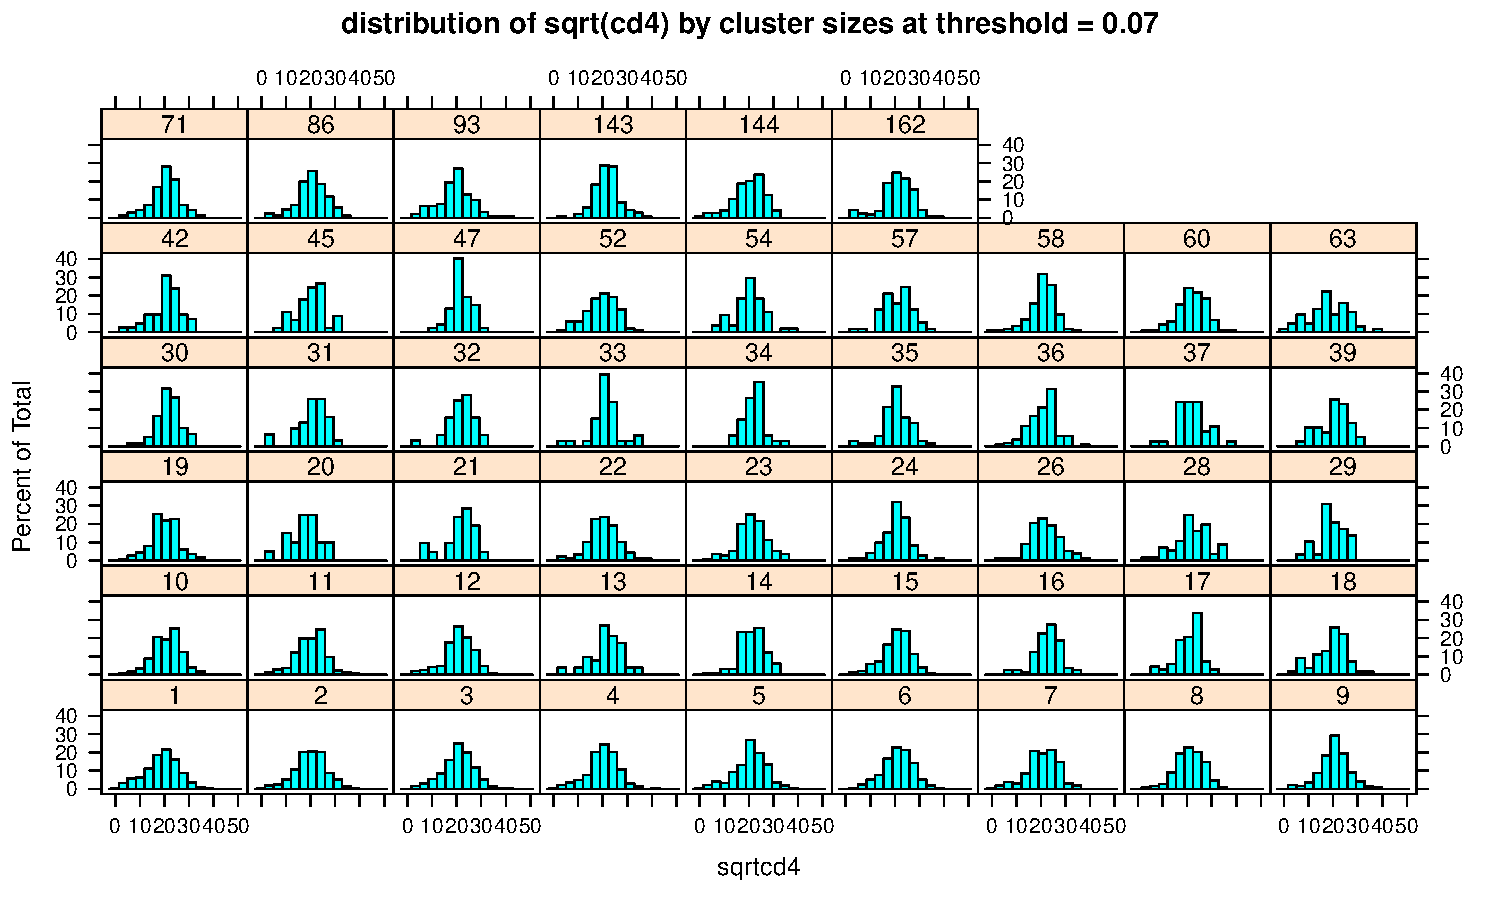
\includegraphics[width=10cm]{figure/plotlattice_UK-1} 
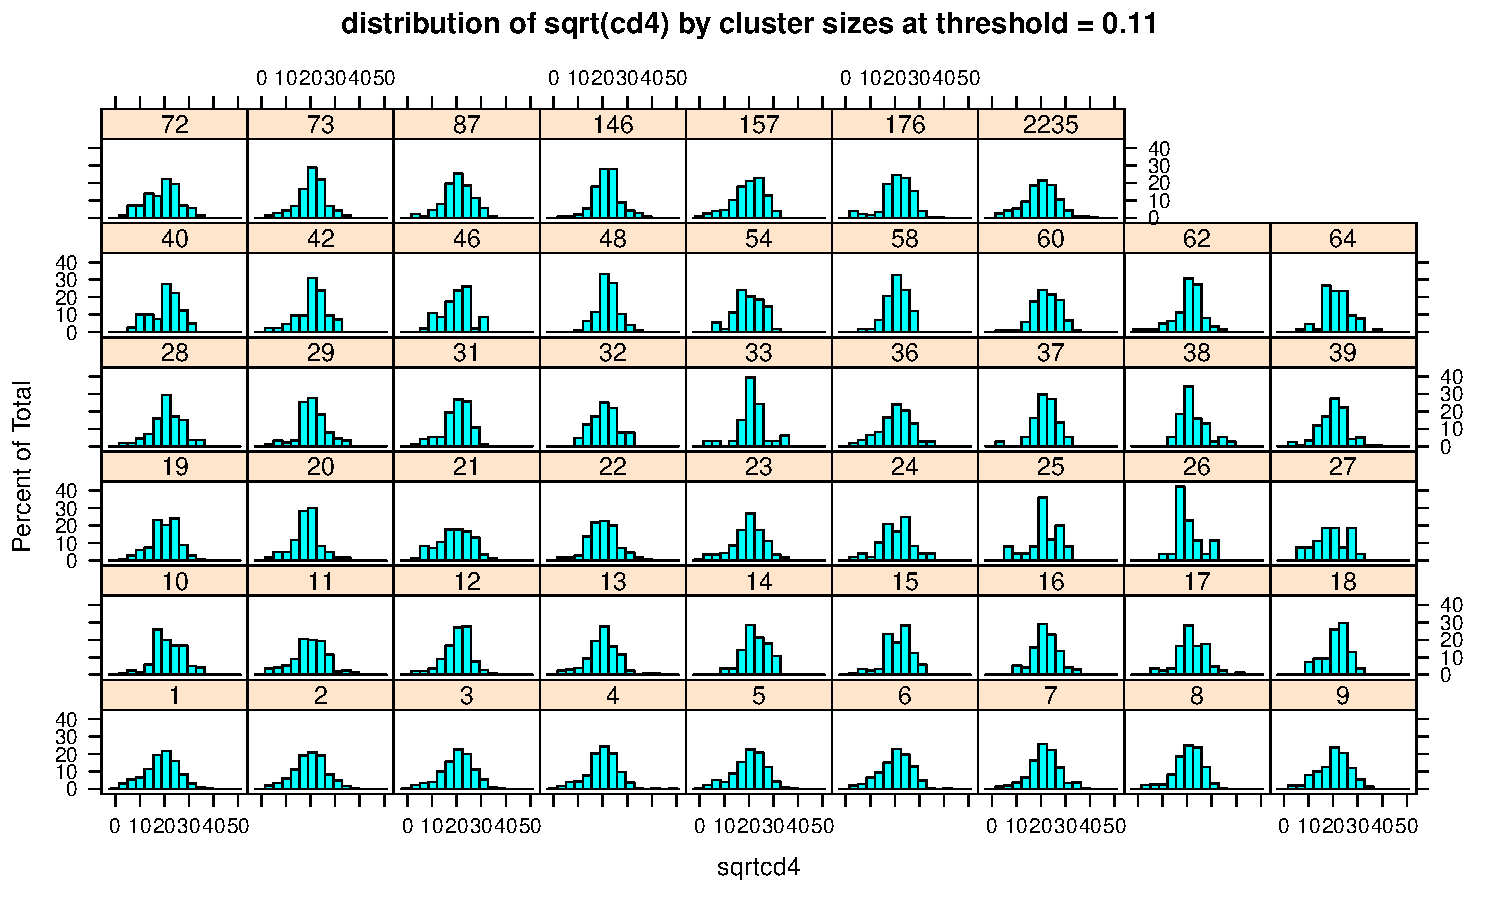
\includegraphics[width=10cm]{figure/plotlattice_UK-2} 
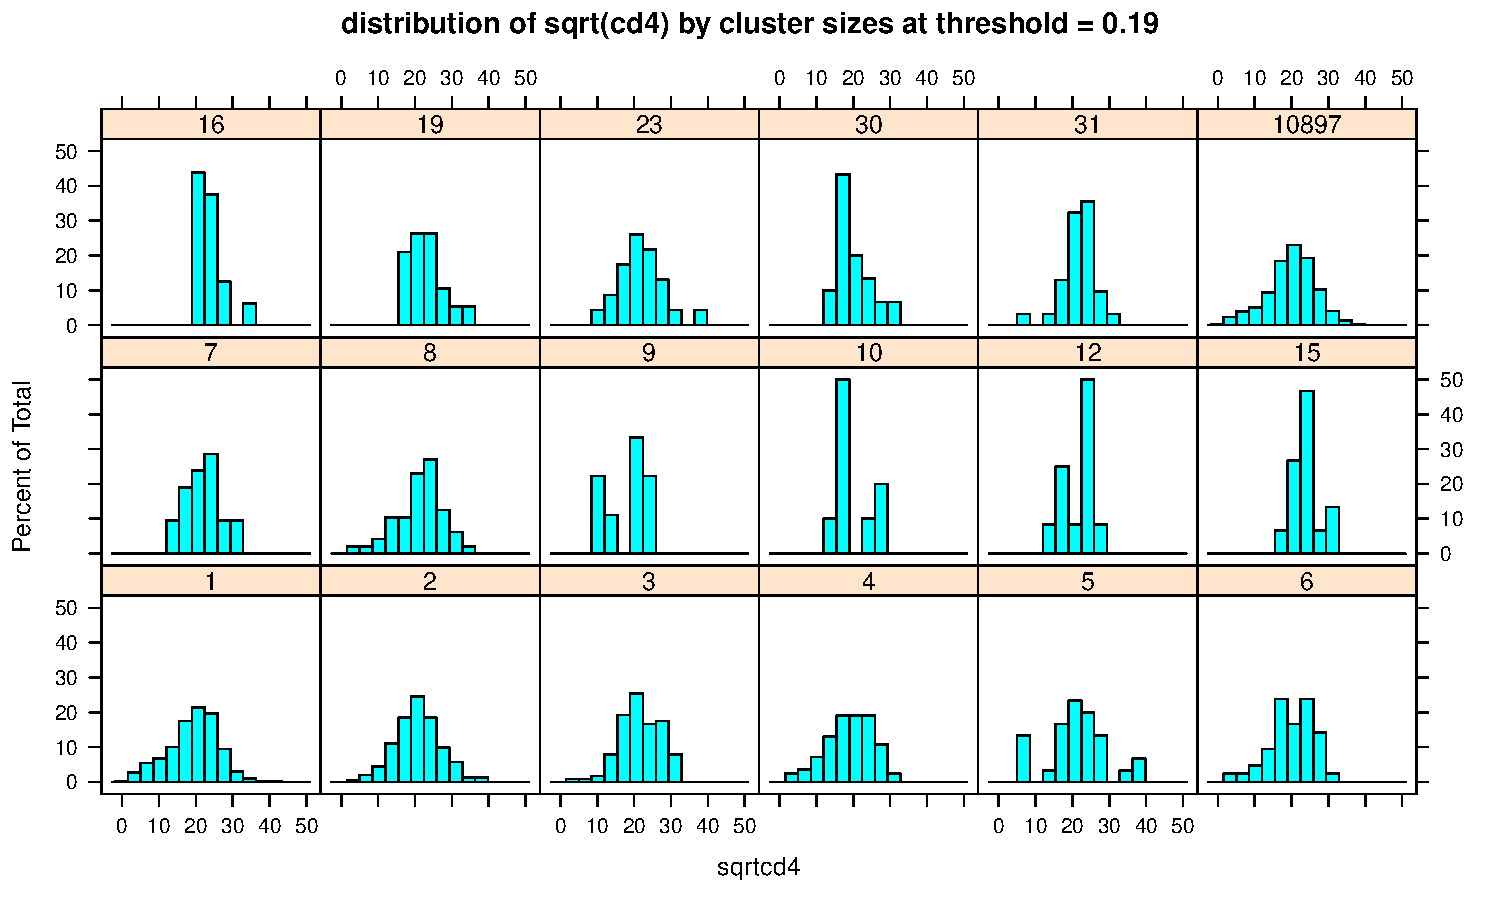
\includegraphics[width=10cm]{figure/plotlattice_UK-3} 
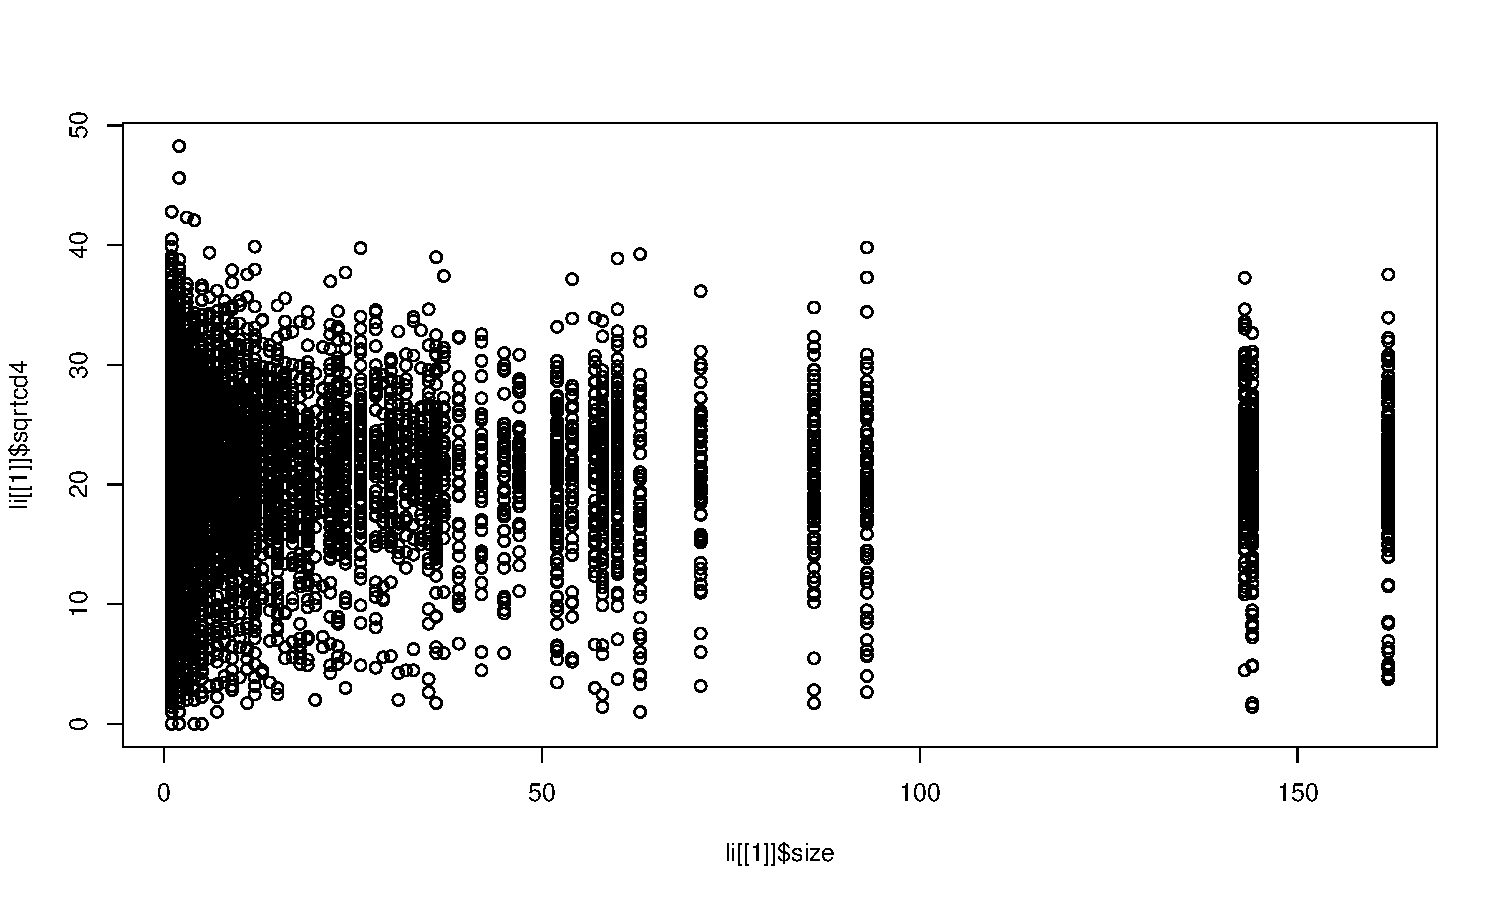
\includegraphics[width=10cm]{figure/plotlattice_UK-4} 

}



\end{knitrout}


\end{document}
